% !TEX options=--shell-escape

\documentclass[12pt]{article}
\usepackage[T1]{fontenc} % Enables \dh and \TH
\usepackage{babel}

\newcommand{\txline}{ \\ }
\newcommand{\customwidth}{ 11.2cm }

\usepackage{titlesec}
\titleformat{\section}
  {\normalfont\normalsize\bfseries}{\thesection.}{1em}{}
\titleformat{\subsection}
  {\normalfont\normalsize\bfseries\itshape}{\thesubsection.}{1em}{}
\titleformat{\subsubsection}
  {\normalfont\normalsize\itshape}{\thesubsubsection.}{1em}{}
\usepackage{geometry}
 \geometry{
 a4paper,
 left=30mm,
 top=25mm,
 bottom=25mm,
 right=30mm}

\usepackage{titling}
\usepackage[capposition=top]{floatrow}

\usepackage{amssymb}

\usepackage{graphicx}

\usepackage[normalem]{ulem}
\useunder{\uline}{\ul}{}

\usepackage{siunitx}
\usepackage{booktabs}
\usepackage{float}
\usepackage{caption}
\usepackage[section]{placeins}
\usepackage{longtable}
\usepackage{multirow}
\usepackage{makecell}
\usepackage{pdflscape}
\usepackage{setspace}
\usepackage{dcolumn}
\usepackage{amsthm}

\usepackage[round, sort]{natbib}
\bibliographystyle{chicago}

\usepackage{authblk}

\usepackage{tabularray}
\usepackage{threeparttable}
\usepackage[hidelinks]{hyperref}  %hyperref still needs to be put at the end!

\usepackage{doi}

\title{Brand Transformation in European Politics:\\ The Rise and Limits of Nonclassical Names}

\author[1, 2]{Endre Borbáth}
\author[2, 3]{Swen Hutter}

\affil[1]{Heidelberg University}
\affil[2]{WZB Berlin Social Science Center}
\affil[3]{Freie Universit\"at Berlin}


\date{} 

\setcounter{secnumdepth}{0} % sections are level 1

\usepackage{etoolbox}

\newcounter{totfigures}
\newcounter{tottables}

\providecommand\totfig{} 
\providecommand\tottab{}

\makeatletter
\AtEndDocument{%
  \addtocounter{totfigures}{\value{figure}}%
  \addtocounter{tottables}{\value{table}}%
  \immediate\write\@mainaux{%
    \string\gdef\string\totfig{\number\value{totfigures}}%
    \string\gdef\string\tottab{\number\value{tottables}}%
  }%
}
\makeatother

\pretocmd{\chapter}{\addtocounter{totfigures}{\value{figure}}\setcounter{figure}{0}}{}{}
\pretocmd{\chapter}{\addtocounter{tottables}{\value{table}}\setcounter{table}{0}}{}{}


\newcommand\hl{\bgroup\markoverwith
{\textcolor{yellow}{\rule[-.5ex]{.1pt}{2.5ex}}}\ULon}

\begin{document}
\sloppy

\begin{titlepage}

\maketitle

\begin{abstract}

\noindent{Political parties in Europe are undergoing profound transformations, with many abandoning traditional brands. This study analyzes party names as indicators of programmatic and organizational change, combining an original content analysis across 28 European countries (1945-2023) with two conjoint survey experiments. We find that ``nonparty'' names have become the majority, reflecting a shift away from ideology toward alternative forms of identification. While movement names appear in wave-like patterns linked to protest cycles, such as after the 2008 Great Recession, nonclassical names are especially prevalent among new, opposition, and right-wing parties. However, a paradox emerges: despite their growing adoption, nonclassical names do not easily yield the anticipated electoral benefits, as new parties seem to gain little from abandoning classical naming conventions. By tracing long-term naming trends and integrating survey experimental evidence, we advance debates on party transformation, political branding, and the evolving interplay between electoral and movement politics in contemporary democracies.}
\end{abstract}

\vspace*{0.5cm}
\noindent \textbf {Keywords:} \emph{political parties, party brands, political crisis, conjoint experiments, Europe}
\vspace*{0.5cm}

\thispagestyle{empty}

\end{titlepage}

\doublespacing

\section{Introduction}

Political parties in Europe are facing profound transformations and challenges, often described as a crisis \citep[][]{Mair_2013}. The partisan landscape is undergoing significant shifts, driven by the rise of new challenger parties that act as issue entrepreneurs, advocating for wedge issues such as immigration and European integration \citep[][]{deVries_Hobolt_2020, de_Wilde_Koopmans_Merkel_Strijbis_Zurn_2019}. This rise is restructuring political conflict as established parties struggle to adapt to shifting preferences and expectations among the electorate \citep[][]{Hooghe_Marks_2018, Kriesi_et_al_2008, Kriesi_et_al_2012}. Many of these challenger parties also embody populist sentiments, mobilizing frustration against the perceived disconnect between elites and the masses \citep[][]{Mudde_2007, Van_Kessel_2015}. Additionally, movement parties are emerging, proposing alternative models of political organization that blur the boundaries between electoral politics and grassroots mobilization \citep[][]{della_Porta_et_al_2017, Castelli_Gattinara_Pirro_2024}. Together, these shifts challenge traditional ideologies and organizational structures that have long defined political parties, marking a significant move away from classical party brands.

Party names serve as crucial indicators of these changes, encapsulating the core of a party's branding. As \citet[][]{Epstein_1966} aptly observed, a party's name constitutes ``the crucial defining element'' of its identity, offering insights into its operational logics and strategic position. Notable examples, such as Podemos in Spain, the Five Star Movement in Italy, Renaissance in France, Law and Justice in Poland, and the Alternative for Germany, illustrate this trend. The systemic move away from traditional naming conventions signals a broader evolution in political branding, mainly driven by new party entry. Yet, despite these visible shifts, analyses of the prevalence and implications of these naming practices remain scarce.

Existing research on party names (or labels) has primarily examined the prevalence of renaming in European democracies. For instance, \citet[][]{Kim_Solt_2017} indicate that approximately one-third of all parties have undergone name changes since 1945. Renaming occurs more frequently among parties with shorter histories, who invest less in established identities, and those facing electoral setbacks, especially in less institutionalized party systems \citep[see also][]{Avina_Spoon_2024, Casiraghi_Cusumano_Chryssogelos_2023, Ibenskas_Sikk_2017}. \citet[][]{Gouglas_Katz_Maddens_Brans_2021} found that parties that change their names are more likely to experience legislative turnover, while \citet[][]{Avina_2023} suggests that rebranding can potentially increase electoral support. These findings indicate that name changes are significant markers of broader organizational transformations, linking party identity to electoral dynamics and stability.

Despite these insights, no study has systematically examined the content of party names and their changes over time. This paper presents the first comprehensive content-based analysis of party names across a long-term framework, covering 28 European countries from 1945 to 2023. Our analysis of the supply side of party names is supplemented by two conjoint experiments embedded in an individual-level population survey conducted in Austria, Germany, Italy, and Hungary in 2023. We investigate three interrelated research questions: First, we assess the extent to which European party systems have moved away from classical naming conventions since the Second World War. Second, we study the conditions under which parties adopt nonclassical names and identify the types of parties that are most likely to do so. Lastly, we examine citizens' preferences and the electoral implications of nonclassical names.

By adopting a content-based approach to party names and distinguishing between programmatic and organizational references, we conceptualize the types of identifiers likely to become more prevalent during periods of party crisis, when parties can no longer claim their role as primary intermediaries in representative democracy \citep[][]{Mainwaring_et_al_2006, Mair_2013, Lupu_2016}. From a programmatic perspective, we argue that weakening ties between parties and their traditional electoral bases correlate with a decline in ideological labels linked to classical party families. In adapting to fragmented societies, parties tailor their appeals to increasingly diverse social groups, often without explicitly referencing these ideological traditions.

From an organizational perspective, we contend that a large share of parties no longer identify themselves as ``parties'' due to the burdensome connotations of the term. Drawing on the literature on party-social movement interactions \citep[][]{della_Porta_et_al_2017, Pirro_Gattinara_2018, Tarrow_2021, Castelli_Gattinara_Pirro_2024}, we suggest that parties increasingly reference horizontal organizational structures, positioning themselves as allies of civil society and nonelectoral street mobilization. By incorporating movement references into their names, they evoke bottom-up, horizontal frameworks.

Our findings demonstrate a substantial increase in the proportion of political parties that avoided the term ``party'' in their names or references to traditional ideologies, a trend that has accelerated since the 1960s. By the early 2020s, nearly two-thirds of European parties no longer identify as ‘parties’ in their official name. The uptake of movement references follows a wave-like pattern, mirroring key protest cycles and crises, such as those triggered by the 2008 Great Recession. The rise of nonclassical names correlates with indicators of party system instability, particularly electoral volatility. On the party level, the trend is primarily driven by the entry of new, right-wing, and opposition parties. Radical right-wing parties go further, frequently adopting names with explicit movement connotations. However, this shift reveals a paradox: despite the increasing use of nonclassical names, they do not generate the expected electoral benefits. Our conjoint experiments suggest that new parties do not gain a significant advantage from adopting nontraditional names, while established parties risk electoral penalties when rebranding.

In the following sections, we introduce our theoretical framework, referencing studies on party branding, the crisis of representation, and citizen preferences. Based on these discussions, we present our hypotheses that structure the presentation of the results: (i) the temporal dynamics of party names, (ii) the profiles of parties likely to adopt nonclassical names, and (iii) citizen responses to these transformations.

\section{Theoretical considerations}

\subsection{From party brands to party names}

Just as brands differentiate products in market competition, they also serve to distinguish political parties in electoral competition. Brands operate as a shortcut, formed in interaction between firms and consumers \citep{Kornberger_2010}. Branding results from strategic investment by leadership but is not solely top-down; it is also shaped through the experiences and perceptions of consumers \citep{Clifton_2009}. In political contexts, brands help parties communicate both identity and competence \citep[for an overview:][]{Ishiyama_Rybalko_2023}. According to \citet{Scammell_2015}, brands in party politics are multidimensional constructs that combine substantive policy positions and performance (boundary conditions) with emotional, cultural, and symbolic appeals (brand differentiators) that arise in interaction between party elites and voters.

However, the concept of party brands is often discussed metaphorically, without a clear empirical indicator. \citet{Kim_Solt_2017} suggest party names as an indicator of branding. They examine the extent of party name changes and demonstrate that renaming is not uncommon. Across European democracies, roughly a third of all parties have renamed themselves at least once since 1945. As stated, parties with a shorter history are more likely to undergo renaming, which reflects lower investment in an existing brand and reaction to electoral setbacks, with significant contextual differences between more institutionalized and weaker party systems \citep[see also:][]{Ibenskas_Sikk_2017, Casiraghi_Cusumano_Chryssogelos_2023, Avina_Spoon_2024}.

Additional studies considering name change as an independent variable have demonstrated its significant consequences for parties' organizational dynamics and electoral success. For example, \citet{Gouglas_Katz_Maddens_Brans_2021} show that parties that change their names are more likely to experience legislative turnover and renew the composition of their parliamentary groups. \citet{Avina_2023} examines the effect of rebranding on electoral performance and finds that parties that rename themselves tend to gain approximately 0.74 percentage points more in vote share than their previous results. In contrast, he does not find a similar effect of electoral punishment for programmatic changes in party manifestos. \citet{Ishiyama_Marshall_2017} identify renaming by former rebel groups as a critical stage in democratization in post-conflict settings, as previously violent groups transition into electoral parties. Overall, these studies indicate that party (re-)naming is not random but rather a strategic choice with meaningful consequences for a party's trajectory.

While these studies emphasize the external outcomes of name change, they also identify a key mechanism related to internal organizational constraints that shape whether and how such transformations occur. As \citet{Ishiyama_Marshall_2017} and \citet{Ishiyama_Rybalko_2023} argue, the extent to which party leaders must accommodate internal factions and constituencies, following the logic of nested games \citep{Tsebelis_1991}, significantly shapes the branding strategies parties can adopt. Leaders cannot unilaterally change a party’s brand; instead, they must negotiate with members who may be deeply invested in the party’s existing name and broader identity \citep{Lupu_2016}. This focus on organizational constraints underscores that rebranding is not merely a strategic act aimed at external audiences, but a negotiated process shaped by internal dynamics.

Another strand of literature examines party names, including those of newly formed parties, as a central element in communicating a party's appeal. Parties enter the public sphere through their name, which is how elites and voters refer to them and how they appear on the ballot. Names are often complemented by additional symbols, such as logos and specific color schemes \citep{Casiraghi_Curini_Cusumano_2022, Casiraghi_Cusumano_Chryssogelos_2023, Avina_Spoon_2024}. \citet{Dolinsky_2022} provides a dataset of group appeals in party names in Israel and the Netherlands between 1977 and 2015. She finds that 44 percent of Dutch parties and about a third of Israeli parties include a group appeal in their name, most often a religious reference. Similarly, \citet{Ishiyama_Breuning_2011} study ethnic parties in post-communist countries and show that parties that do not include an ethnic group's name tend to be more inclusive, attract some support from the majority group, and are more likely to encourage their supporters to accept the democratic framework of the nation-state they inhabit.

This body of literature faces three key limitations that we aim to address: (i) the lack of a systematic content-based perspective, (ii) an exclusive focus on the electoral arena, and (iii) insufficient evidence on the electoral consequences of party names. We address the first two limitations by analyzing references in party names along two dimensions: programmatic and organizational. The programmatic dimension captures the extent to which party names explicitly reference the ideological traditions of established party families, such as Christian democrats, socialists, liberals, and conservatives. These party families have historically structured political competition and played a key role in integrating European societies after World War II \citep[e.g.,][]{Kirchheimer_1966}. However, as societies become more fragmented and electoral competition intensifies, parties may strategically abandon explicit ideological markers in their names to attract a broader electorate with weaker partisan ties and less attachment to historically dominant ideological traditions.

The organizational dimension, by contrast, concerns the organizational model and identity referenced in a party's name. As the crisis of political parties deepens, some parties may move away from explicitly calling themselves a ``party,'' instead opting for alternative organizational labels that may appear more attractive. Building on the emerging literature on party-movement interactions and movement parties \citep[e.g.,][]{della_Porta_et_al_2017, Pirro_Gattinara_2018, Tarrow_2021, Castelli_Gattinara_Pirro_2024}, we argue that references to horizontal organizational structures associated with movement politics may be perceived as a more viable alternative to the traditional party model. Rather than considering electoral competition in isolation, we argue that parties position themselves as potential allies of civil society, social movements, and other actors engaged in nonelectoral mobilization.

Building on the distinction between ideological and organizational dimensions, we develop a novel typology that classifies party names along a continuum from classical to nonclassical. We propose a typology that distinguishes six mutually exclusive categories: 1) classical party names (e.g., the Conservative and Unionist Party in the UK), 2) ideological nonparty names (e.g., the Christian-Democratic Union in Germany), 3) ideological movement names (e.g., the Panhellenic Socialist Movement in Greece), 4) nonideological party names (e.g., the Democratic Party in Italy), 5) nonideological nonparty names (e.g., Law and Justice in Poland), and 6) nonideological movement names (e.g., the Five Star Movement in Italy). From these six categories, we focus empirically in particular on classical party names at one end of the continuum, nonideological movement names at the other, and nonideological nonparty names as an intermediate category within the nonclassical spectrum.

To address the third limitation in the literature, we examine the demand-side consequences of party name choices and investigate the causal effect of party names on electoral appeal using two survey experiments. In line with existing research, we distinguish between newly established party names and name changes among existing parties.

Before outlining our research design, we first theorize how the crisis of representation may shape party name choices, identify the parties most likely to adopt nonclassical names, and discuss the expected electoral consequences of these strategic naming decisions.

\subsection{Why shift to nonclassical names? The crisis of representation}

Academic literature and public discourse increasingly argue that liberal democracies are in crisis. In some cases, democratic backsliding is evident, driven by authoritarian forces that weaken liberal checks and balances \citep[e.g.,][]{McCoy_Rahman_Somer_2018, Bohle_Greskovits_Naczyk_2024}. In other cases, the crisis remains latent, yet to fully materialize \citep[e.g.,][]{Valgardsson_Jennings_Stoker_Bunting_Devine_McKay_Klassen_2025}. A key aspect of this crisis is the declining ability of mainstream parties to connect citizens with the state \citep[e.g.,][]{Mair_2013, Schmitter_2001, Katz_Mair_1995}. As the mass party model declined \citep{Duverger_1954}, parties withdrew from representing distinct societal milieus. Since the 1960s, they have increasingly positioned themselves as catch-all organizations, appealing to broad electorates rather than specific groups \citep{Kirchheimer_1966}. This crisis of democratic representation has both attitudinal (distrust and perceived misrepresentation) and behavioral (declining electoral participation) dimensions \citep{Mainwaring_et_al_2006}. Kirchheimer's \citeyearpar{Kirchheimer_1966} diagnosis, that parties are losing their role as intermediaries between citizens and government, has thus only become more relevant since he originally formulated it.

The crisis of representation unfolds through both structuralist and functionalist dynamics. From a structuralist perspective, the crisis stems from mainstream parties' inability to adapt to shifting cleavage structures, as they face competition from both the radical right and the new left \citep{Hooghe_Marks_2018, Kriesi_et_al_2008, Kriesi_et_al_2012}. A key empirical indicator of this crisis is programmatic convergence, which dilutes party brands, making it harder for voters to distinguish between electoral alternatives. This increases uncertainty and weakens retrospective accountability. Several factors drive this process, including exogenous shocks \citep{Lupu_2016, Hutter_Kriesi_2019}, incumbency \citep{Roberts_2014}, electoral losses \citep{Janda_Harmel_Edens_Goff_1995}, and intra-party conflicts \citep{Pasotti_2010}. For instance, \citet[][]{Lupu_2016} argues that brand dilution led to the electoral collapse of established parties in Latin America. Mainstream parties, particularly under economic pressure, converged in their appeals, incentivizing incumbents to deviate from party lines in favor of pragmatic policymaking \citep[see also:][]{Roberts_2014}. However, this inconsistency deepens dissatisfaction with democracy and contributes to declining turnout rates \citep{Dass_McAll_2020}.

From a functionalist perspective, the crisis is reflected in the increasing volatility and fragmentation of party systems, as well as the growing success of new parties \citep{Bertoa_Enyedi_2021, Dassonneville_2022, Haughton_Deegan_Krause_2020, Engler_2023}. From this perspective, the crisis of mainstream parties is linked to their organizational brand: long-established governing parties struggle against emerging challengers \citep{deVries_Hobolt_2020, Sikk_2011, Haughton_Deegan_Krause_2020}, which mobilize against the perceived aloofness of established parties \citep[][]{Mudde_2007, Van_Kessel_2015}. Electoral volatility, often taken as a key empirical indicator, signals parties' difficulty in maintaining stable voter bases \citep{Dalton_Wattenberg_2000}. This is particularly concerning when volatility entails ideological shifts \citep{Dassonneville_2022} or the rise of new parties \citep{Haughton_Deegan_Krause_2020, Engler_2023}. High volatility is also associated with weak party system institutionalization \citep{Bertoa_Enyedi_2021}, undermining retrospective accountability when voters cannot reward or punish parties that may not survive until the next election \citep{Borbath_2021}.

One consequence of this crisis of representation and the broader hollowing out of democracies \citep{Berman_2021, Mair_2013} is the normalization of protest participation \citep{Meyer_Tarrow_1998, giugni_grasso_2019a}. Participation outside of political parties, such as attending demonstrations, has become a widely accepted form of civic engagement, influencing norms of citizenship and political involvement \citep{Dalton_2008b}. As demonstrations and other protest activities increasingly complement or substitute voting \citep{oser2022protest, rojon2025comparing}, parties are incentivized to adapt their organizational form and public image. Many new parties, in particular, turn to the protest arena as a source of organizational innovation \citep{della_Porta_et_al_2017, Tarrow_2021, Castelli_Gattinara_Pirro_2024}, contributing to the erosion of boundaries between electoral and protest politics. This convergence creates a strategic rationale for new entrants to avoid classical “party” labels. Emphasizing horizontal, flexible, and citizen-oriented organizational models, they seek to distance themselves from hierarchical and elite-driven connotations associated with traditional party identities. In this context, movement names become a tool for signaling proximity to grassroots mobilization. Classical labels, by contrast, may evoke institutional inertia or reinforce the crisis of representation, making them less attractive to voters. As such, the shift toward movement names might reflect a calculated effort to frame the party's brand in ways that carry electoral appeal.

Drawing on this discussion, we formulate our first expectation: as the crisis confronting political parties deepens, and as many seek to define themselves in less hierarchical or ideologically rigid ways, the composition of party systems increasingly reflects a shift toward parties with nonclassical names. For clarity, classical party names reference both a traditional organizational label (i.e., “Party”) and an established ideological anchor (e.g., Christian Democrat, Conservative, Socialist). In contrast, nonclassical names signal a break with these conventions. In more formal terms, we expect that:

\begin{quote}
\textit{H1: Compared to post-Second World War party systems, present-day party systems are more likely to feature a higher proportion of political parties that do not have classical party names.}
\label{hyp:party_system}
\end{quote}

\subsection{Who adopts nonclassical names? Challenger vs. mainstream parties}

The long-term transformation of European party systems, unfolding against the background of the crisis of representation, does not affect all parties in the same way. Parties respond differently to these crisis conditions. Challenger parties, less constrained by entrenched organizational and programmatic legacies, can adapt their brand more easily, while mainstream parties tend to be slower to respond. Therefore, challenger parties are expected to play a key role as vanguards of this transformation. As already emphasized in the discussion of H1, this party-level dynamic, particularly the strategic behavior of new entrants, drives broader party system change over time. However, conceptualizing the challenger status differs between the structuralist and functionalist perspectives introduced above.

The structuralist tradition points to the importance of ideological factors, highlighting political parties that challenge mainstream parties programmatically and politicize issues previously absent from electoral dynamics \citep{Hooghe_Marks_2018, Kriesi_et_al_2008}. The issues that challenger parties mobilize, such as immigration, European integration, and climate change \citep[][]{deVries_Hobolt_2020, de_Wilde_Koopmans_Merkel_Strijbis_Zurn_2019, Dickson_hobolt_2024}, cut across the preferences of the mainstream party landscape. From this perspective, the challenger status is primarily associated with the radical right and green/new left party families, which do not integrate neatly into the traditional left-right dimension. As the issues they politicize have gained importance in the shadow of Europe's multiple crises \citep{Hutter_Kriesi_2019, Hooghe_Marks_2018}, radical right and green parties have increased in popularity, further challenging their mainstream competitors and heightening the fragmentation of European party systems.

By contrast, the functionalist perspective is less concerned with parties' ideological positions and focuses more on their strategic position in the party system \citep[e.g.,][]{Bertoa_Enyedi_2021}. By classifying parties as dominant or challenger based on whether they had previously entered government, \citet{deVries_Hobolt_2020}, for instance, document an electoral shift in Western Europe over time from dominant to challenger parties. While \citet{deVries_Hobolt_2020} emphasize that programmatic positioning also plays a role, \citet{Sikk_2011} proposes that ``newness'' in itself can be a winning formula for challengers. Through a comparative analysis of four Eastern European parties, Sikk shows that new parties can succeed even when they occupy the same ideological position as previously existing parties or, as \citet{Engler_2023} finds, when they do not take a clear position on the main divides structuring the party system. Similarly, \citet{Haughton_Deegan_Krause_2020} distinguish between old and new parties, identifying the emergence of new parties in Central and Eastern Europe as posing the main challenge to established parties.

The literature on the interactions between movement and electoral politics integrates insights from both the structuralist and functionalist perspectives. In terms of ideology, radical right \citep[e.g.,][]{Castelli_Gattinara_Pirro_2024} and green/new left parties \citep[e.g.,][]{Blings_2020, della_Porta_et_al_2017} have featured prominently in these analyses. \citet{Kitschelt_2006}, for example, points to radical right and green parties as archetypal “movement party entrepreneurs,” which invest little in resolving collective and social choice problems. In other words, these parties are less likely to invest in organizational hierarchies that constrain leaders, and are also less likely to adapt encompassing electoral programs. In addition, this research strand also examines factors typically associated with a functionalist perspective. In this regard, studies indicate that opposition status is the main predictor of a party's engagement with ``street'' mobilization \citep{Hutter_Vliegenthart_2018}. Particularly in Central and Eastern European countries, parties that belong to the mainstream or the challenger party families are likely to mobilize when they are in opposition \citep{Borbath_Hutter_2021}.

To summarize, the literature points to several party-level features associated with breaking from classical party names. These include newness, opposition status, and membership in challenger party families (e.g., radical right, green). By omitting ideological labels or established organizational tags like “party,” these challengers signal their alternative approach and outsider status. Accordingly, we formulate our second hypothesis as follows:

\begin{quote}
\textit{H2: Newly founded parties, long-term opposition parties, and those belonging to challenger party families (i.e., radical right, green) are more likely to adopt nonclassical party names than their respective competitors.}
\label{hyp:party_level}
\end{quote}

\subsection{How do nonclassical names influence voters? A demand-side perspective}

From a demand-side perspective, the literature primarily examines how citizens develop interconnected networks of political information around party brands \citep[e.g.,][]{John_Loken_Kim_Monga_2006, French_Smith_2010}. The brand labels or names serve as informational cues or heuristics, helping voters navigate complex political environments and form structured evaluations of parties \citep{Popkin_1994, Lau_Redlawsk_2001}. As \citet{Snyder_Ting_2002} argue from a theoretical perspective (supported by empirical illustrations), party names play a key role in enabling citizens to hold parties accountable.

From an experimental standpoint, \citet{van_Elk_2010} demonstrate that even left-right spatial metaphors embedded in party names can automatically activate political associations. This activation is also sensitive to a voter's own ideology, suggesting that labels alone can polarize or prime voters' thinking. Along similar lines, \citet{Lau_Redlawsk_2006} provide evidence that voters rely on party labels to reduce cognitive effort, often substituting these heuristics for more detailed information about policy or ideology. However, recent work by \citet{Titelman_Lauderdale_2025} suggests that the marginal effect of party labels may be limited when voters already possess clear information about the ideological positioning of the political supply.

When parties adopt nonclassical brands or names, they may do so based on the assumption that classic labels (e.g., ``Socialist,'' ``Conservative,'' ``Christian Democratic'') have lost their broad appeal, an idea supported by the research on the crisis of representation, declining partisan ties, and voter volatility across Europe \citep{Mair_2013, Dalton_Wattenberg_2000, Kirchheimer_1966, Katz_Mair_1995, Valgardsson_Jennings_Stoker_Bunting_Devine_McKay_Klassen_2025}. This crisis creates conditions for new or challenger parties to exploit the perception of traditional elites as aloof by branding themselves in novel ways \citep[][]{Mudde_2007, Van_Kessel_2015}. Nonclassical names can thus convey novelty or a break from discredited elites, appealing especially to voters who seek alternatives to perceived establishment politics. \citet{Kam_2005} shows, for instance, some voters are more sensitive to cues than others, making nonclassical names potentially especially effective among those who are not anymore attached to established parties.

The case of En Marche! in France illustrates how such naming choices are not accidental, but part of a strategic plan. As Adrien Taquet, the communications advisor behind the name,  recalled, the label was designed to evoke movement, disruption, and emotional resonance with collective marches throughout history, from the French Revolution to the Civil Rights Movement, while also subtly embedding Emmanuel Macron’s initials in the acronym \citep{lorrain2017}. While voters are not misled about whether such a formation is a party, the name was intentionally chosen by Macron's camp to frame their initiative as civic, open, forward-looking, and unaffected by traditional partisan baggage.

A related development is the rise of expressive voting, in which voters do not necessarily base their choice on programmatic or instrumental evaluations of which party best aligns with their ideological preferences. Instead, they may vote in ways that reflect emotional or symbolic attachments, sometimes prompted by charismatic leadership, populist appeals, or distinctive party labels \citep{Brennan_Lomasky_1997, Schuessler_2000, Hamlin_Jennings_2011}. For instance, \citet[][]{Hobolt_Tilley_2014} demonstrate that citizens' group-based predispositions toward the European Union can outweigh standard partisan cues, causing them to shift blame or credit in ways that do not align with traditional loyalties.

In combination, parties' strategic rebranding attempts and citizens' shifting motivations can amplify the power of nonclassical brands. These alternative brands potentially offer narratives of renewal, authenticity, or outsider status. Consequently, nonclassical party names may outcompete classical labels, which are often associated with the status quo or perceived as disconnected from voter realities. Drawing out the individual-level implications of these trends, we hypothesize:

\begin{quote}
\textit{H3: Voters find political parties with nonclassical names more appealing than political parties with classical names, all else being equal.}
\end{quote}

\section{Data and Methods}

\subsection{Study 1: Party names}

One reason researchers have not conducted a comparative study on the content of party names is the lack of a comprehensive dataset on party name changes over a long period. Existing datasets, such as ParlGov \citep{Doring_Manow_2021} or the party manifesto data \citep{Lehmann_et_al_2023}, focus on continuity and track the same parties over the longest timeframe possible, but they do not systematically cover differences in the names of political parties.

Therefore, we undertook a major data collection effort. We used ParlGov as our starting point and manually coded changes in the names of all parties in this dataset. During this process, we relied primarily on Wikipedia to trace the evolution of party names over time, consulting both the English-language Wikipedia pages and the typically more detailed national-language pages of the respective parties. Our focus was on the name under which parties appeared on the ballot paper.\footnote{In the case of countries where ballot papers are printed in multiple languages (e.g., Switzerland), we opted for the name of the party in the most widely spoken language.} To distinguish between new and old parties, we followed ParlGov's decisions on whether a party received a new party ID.\footnote{We applied the same rule to coding mergers, splits, electoral coalitions, and similar organizational transformations \citep{Ibenskas_Sikk_2017}. Coalitions are included only if the parties later split. In other words, names referring exclusively to electoral coalitions are not included. We double-checked the new/old party distinctions with Wikipedia and additional sources and found them to be highly consistent.} Although Wikipedia is widely used in political science \citep{Brown_2011} and in studies of party competition \citep{Herrmann_Doring_2021}, offering comprehensive coverage of political parties, we still wished to validate its information with additional sources. Most importantly, we used internal documents from the party manifesto project \citep{Lehmann_et_al_2023}, as well as secondary literature. The resulting data covers 616 unique parties from 28 European countries between 1945 and 2023. In countries that democratized later, we covered the period starting with the first competitive election.\footnote{We also conduct the analysis separately for Western and Eastern European countries. Most of the observed patterns are consistent across both regions. The main difference is that in Eastern Europe, mainstream parties are generally more likely to adopt nonclassical names. The full results are presented in Appendix C.} We used this dataset to test our over-time hypotheses (H1) and to examine which parties are most likely to adopt nonclassical names (H2).

In classifying party names, we considered both programmatic and organizational references. Among programmatic references, we singled out nonideological references. Importantly, by nonideological references, we do not mean labels devoid of all value content, but rather labels that do not reference historically rooted ideological antagonisms associated with traditional party families. More concretely, these names do not refer to classical party families or ideologies such as socialism, Christian democracy, liberalism, etc. Under nonideological references, we included labels containing an action verb or referencing values, the country's name, the leader's name, anti-elitism, reforms, democracy, the people, or even broader statements.\footnote{To further probe the validity of our classification, we asked an independent coder to assess whether names categorized as nonideological might nonetheless convey an ideological `vibe.' Of the names in this category, approximately 6.9\% (39 in total) were judged to have ideological connotations: 5.45\% were placed on a left-right spectrum, and 3.7\% on a progressive-conservative scale. This perceptual coding, while necessarily subjective, indicates that only a small minority of names in the nonideological category might evoke ideological associations for observers. Since these names are not anchored in historically rooted ideological traditions, we retain them in the nonideological category.} Appendix A, Figure 1 includes more information on the distribution of each of these terms.

Regarding organizational references, we coded both the absence of the term ``party'' in the label and the presence of a movement reference. These two are mutually exclusive: parties that do not call themselves ``party'' may go a step further and adopt a movement label, though not all do so. While ``party'' may be associated with a hierarchical, potentially rigid structure, references to movements evoke more horizontal and inclusive forms of organization. Among movement references, we included names suggesting an image of marching in the streets. Accordingly, we coded ``rally'', ``block'', ``front'', ``forces'', ``force'', ``movement'', ``action'', ``attack'', ``fighters'', ``march'', and ``revolution'' as movement references. Appendix A, Figure 2 shows the prevalence of each of these terms. Drawing on these two dimensions, we define a typology of six possible party name types as previously described. We focus in particular on the prevalence of three of these types: classical party names, nonideological movement names, and nonideological nonparty names.

To explain variation in our three dependent variables, we included several types of party- and context-level information. On the party level, we used the eight party families included in ParlGov: agrarian, Christian democracy, communist/socialist, conservative, green/ecologist, liberal, right-wing, and social democracy.\footnote{We recoded the Swiss People's Party and the (True) Finns Party as radical right parties.} We classify Christian-democratic, conservative, liberal, and social democratic parties as mainstream. To examine differences between new and old parties, we included the logged value of party age.\footnote{In line with other studies, we log party age because we expect a nonlinear relationship between party age and our dependent variables \citep[see also][]{Avina_2023}. We also tested a linear specification of party age, which did not change our interpretations.} For the strategic position, we used a dichotomous indicator marking whether a party had ever held the prime ministership. To address the role of internal organizational constraints, we also examined how branding choices relate to party cohesion and the concentration of leadership power (taking their role in the candidate selection process as a proxy).\footnote{Since these variables are only available for a subset of our data, we present the analysis in Appendix A. The results show that parties with strong leaders are more likely to adopt classical party or nonideological movement names, while highly unified parties are more prone to use nonideological movement names. Conversely, low cohesion is associated with a stronger adherence to classical party names. These findings support the argument that party branding also reflects internal bargaining dynamics rooted in the organizational structure.} Depending on the analysis, we also controlled for current opposition status, vote share, and electoral coalitions.

As contextual information, we added country*year-level indicators typically associated with the crisis of representation and changing party systems. To account for programmatic convergence, we used polarization as the key indicator. Since many studies have shown that electoral competition in Europe is multidimensional \citep[e.g.,][]{Kriesi_et_al_2008, Kriesi_et_al_2012, Hooghe_Marks_2018}, we distinguished between economic and cultural polarization. We measured both dimensions using the party manifesto data \citep{Lehmann_et_al_2023}, employing the same issue classification as \citet[][p.~67]{Hutter_Kriesi_2019} and the formula proposed by \citet[][p.~906]{Dalton_2008a}. As functional features, we included electoral volatility based on the updated dataset of \citet{Emanuele_Chiaramonte_Soare_2020}. We also incorporated turnout in the last national parliamentary elections from the \citet{IDEA_2020} dataset and the quality of electoral democracy index from the V-Dem Country-Year Dataset \citep{Coppedge_et_al_2024} to account for variation in exposure to the crisis of democracy. Finally, we controlled for presidentialism (as opposed to parliamentarism) using the indicator from the Quality of Governance standard dataset \citep{Teorell_et_al_2025}.

All models included period-fixed effects to test our hypotheses on over-time dynamics.\footnote{We also tested our hypotheses using a linear time trend specification and found significant trends over time.} Our periodization follows theoretical considerations about the evolution of European party systems and empirical considerations regarding data density. Specifically, we used 1945 to 1969 as the reference category, then grouped subsequent periods into 1970 to 1989, 1990 to 2008, and 2009 to 2023.

Multiple levels of analysis structured the resulting data: party names were nested within parties and years. We relied on a three-level model, with parties nested in country*years and countries.\footnote{We also applied panel models with party-fixed effects. However, because most parties do not change the type of their brand over their organizational lifecycle (see Appendix B), these models are highly inefficient and do not yield interpretable results.} We sought to capture both name changes and continuity, so we included the ``negative cases'' of no change. To do so, we expanded the dataset so that each party*year combination was present from the first election in which the party participated until its disappearance. Because our dataset comprises the full population of European parties, we focused on substantive effect sizes rather than p-values.

\subsection{Study 2: Survey experiment}

To capture cross-national variation in Europe's crisis of representation, we selected four cases for our survey experiment: Italy, Germany, Austria, and Hungary (see Appendix D for a detailed discussion of case selection). In this study, we focus on similarities across contexts, as we are primarily interested in findings that generalize beyond single country cases.

To examine how party names affect voters' attitudes, we conducted two conjoint survey experiments. The first experiment focused on newly formed parties whose policy positions are programmatically congruent with respondents' own positions.  The second experiment examined the rebranding of currently existing parties supported by respondents. We provide more details on the second experiment in Appendix D and concentrate on the first experiment in the main text. We use these experiments to test our hypothesis on the appeal of nonparty names (H3).

Both experiments were part of a research project on movement brands and also included treatments related to party organizations and mobilization repertoires. We use the results concerning party organizations and mobilization repertoires as a benchmark when assessing the effects of party names. The survey was administered in 2023, with similar sample sizes in all four countries.\footnote{The Austrian survey was fielded earlier (06.02.2023--14.02.2023; n=2110) than the surveys in Italy and Hungary (24.07.2023--01.08.2023; n=2129 and n=2160, respectively), followed by the survey in Germany (08--19.12.2023; n=2936).} It was conducted online by the company Bilendi, using a quota sample representative of each country's population regarding age, gender, and education. The Ethics Committee of WZB Berlin Social Science Center approved the study, and we preregistered both the design and our hypothesis.\footnote{Available at \url{https://osf.io/zxunh/?view_only=d439092c947a48c5ae405ab0bf69b5e8}.}

We designed the experiment to simulate the entry of a new party into the respective country's parliament. The fictitious new party advocated policy positions that were programmatically congruent with respondents' preferences (see Appendix D). We employed these congruent issue positions to isolate the marginal effect of the party's brand from its programmatic alignment, even though this approach may reduce the likelihood of detecting large effects \citep{Titelman_Lauderdale_2025}.

Respondents were then shown two profiles (Group A and Group B), which read:

\singlespacing
\begin{table}[H]
\small
\centering
\caption*{}
\begin{tabular}{ll} 
\toprule
\textbf{Group A} & \textbf{\textbf{Group}~B} \\ 
\midrule
\begin{tabular}[c]{@{}l@{}}A new political group is coming to the \\\textless{}name of the country's parliament\textgreater{}\\with the promise to fight for \\\textless{}program\textgreater{}!\\\\~ -~ The group calls itself \textless{}name\textgreater{}\\~ -~ \textless{}Organization\textgreater{}\\~ -~~It promises \textless{}action form\textgreater{} to~\\~ ~ ~represent its program.\\\\This new force needs the support of \\people like you!\end{tabular} & \begin{tabular}[c]{@{}l@{}}A new political group is coming to the \\\textless{}name of the country's parliament\textgreater{}\\with the promise to fight for \\\textless{}program\textgreater{}!\\\\~ -~~The group calls itself \textless{}name\textgreater{}\\~ -~ \textless{}Organization\textgreater{}\\~ -~~It promises \textless{}action form\textgreater{} to~\\~ ~ ~represent its program.\\\\This new force needs the support of \\people like you!\end{tabular} \\
\bottomrule
\end{tabular}
\end{table}
\doublespacing

The two profiles were randomly generated from predefined values, including the order of the three bullet points. Table \ref{exp_1_values} presents the predefined values:

\singlespacing
\begin{table}[H]
\small
\centering
\caption{Design of the new party branding conjoint experiment},
\label{exp_1_values}
\begin{tblr}{
  cell{2}{1} = {r=3}{},
  cell{5}{1} = {r=3}{},
  cell{9}{1} = {r=3}{},
  vlines,
  hline{1,5,8-9,12} = {-}{},
  hline{2} = {-}{0.08em},
  hline{3-4,6-7,10-11} = {2-3}{},
}
\textbf{Attribute} & \textbf{Level} & \textbf{Formulation}\\
Name & None & \textbf{New \textless{}Country name\textgreater{}}\\
 & Party & \textbf{Party for a New~\textless{}Country name\textgreater{}}\\
 & Movement & \textbf{Movement for a New \textless{}Country name\textgreater{}}\\
Organization & None & empty\\
 & {Movement party \\organization} & {The new group maintains close ties with~\\\textbf{civil society organizations~}and has a\\strong presence of \textbf{active members} at\\the local level.}\\
 & {Media party \\organization} & {The new group has \textbf{a strong personality}\\at the top and communicates intensively \\via \textbf{classic and social media}.}\\
 Program & Congruent & {Depending on previous answers:\\\labelitemi\hspace{\dimexpr\labelsep+0.5\tabcolsep}less welfare state benefits and less taxes\\\labelitemi\hspace{\dimexpr\labelsep+0.5\tabcolsep}more welfare benefits and more taxes\\\labelitemi\hspace{\dimexpr\labelsep+0.5\tabcolsep}facilitating the immigration of foreigners\\\labelitemi\hspace{\dimexpr\labelsep+0.5\tabcolsep}restricting the immigration of foreigners\\\labelitemi\hspace{\dimexpr\labelsep+0.5\tabcolsep}a stronger climate protection policy\\\labelitemi\hspace{\dimexpr\labelsep+0.5\tabcolsep}a less far-reaching climate protection policy}\\
Repertoire & None & empty\\
 & Demonstrations & {to take the fight outside of parliament and \\organize~\textbf{public demonstrations}}\\
 & Parliament & {To focus on their work and advances \\in \textbf{parliament}}
\end{tblr}
\end{table}
\doublespacing

Each treatment included an empty, reference category, which served as a baseline comparison. We used the four name-treatment values -- (1) empty, (2) New [Country name], (3) Party for a New [Country name], and (4) Movement for a New [Country name] -- to evaluate our hypothesis. Respondents were asked to evaluate two profiles three times.

To measure our dependent variables, respondents answered two items after both experiments. First, they rated their support for the two profiles on a scale from 0 to 10 (\emph{``How much do you support the described group/scenario `A/B'?''}). Second, they chose between the two profiles: \emph{``Which of the two organizations/scenarios would you be more likely to vote for?''} Our results remain robust across both measurement techniques. In the main text, we focus on the choice (trade-off) item; see Appendix E for the results based on the continuous scale. Following our preregistration, we also performed additional analyses of heterogeneous effects by satisfaction with democracy, left-right ideology, strength of party identification, history of participation in demonstrations, internal and external political efficacy, populist attitudes, trust, and the issues on which respondents self-selected into treatment groups (positions and salience) (see Appendix E).

\section{Results}

\subsection{Trends in party naming (1945-2023)}

We first examine the over-time dynamic of the prevalence of party names, classified according to the ideological and organizational dimensions.\footnote{In Appendix A, Figure 3, we include the over-time distribution of all six types, distinguished in our typology. Here, we opted for the more parsimonious presentation, but our interpretation applies to both types of figures.} For this, we only focus on the Western European countries that we can observe for the entire period between 1945 and 2023.\footnote{However, the substantive conclusions also hold for Eastern Europe, where the trend lines follow similar patterns, albeit at generally higher levels, and the overall distribution of party name types is likewise comparable across the two regions (see Figure 1-2 in Appendix C).} Figure \ref{Fig:timeline} presents the results.

In line with H1, the figure shows the progressive increase in nonclassical names. This confirms that the abandonment of explicit ideological anchors or “party” labels has become more widespread. In doing so, parties appear to have responded to the crisis of representation since the end of the late 1960s. We observe an almost linear trend of increasingly more parties having a nonideological name. While in 1965 20\% of names were nonideological, their share more than doubled by the second half of the 2010s. Similarly, we observe a steady increase in nonparty names, particularly since the second half of the 1980s. In 1985, about one-third of party names did not include a party reference. The share of such nonparty names increased to more than 50\% by 2020.

\begin{figure}[H] 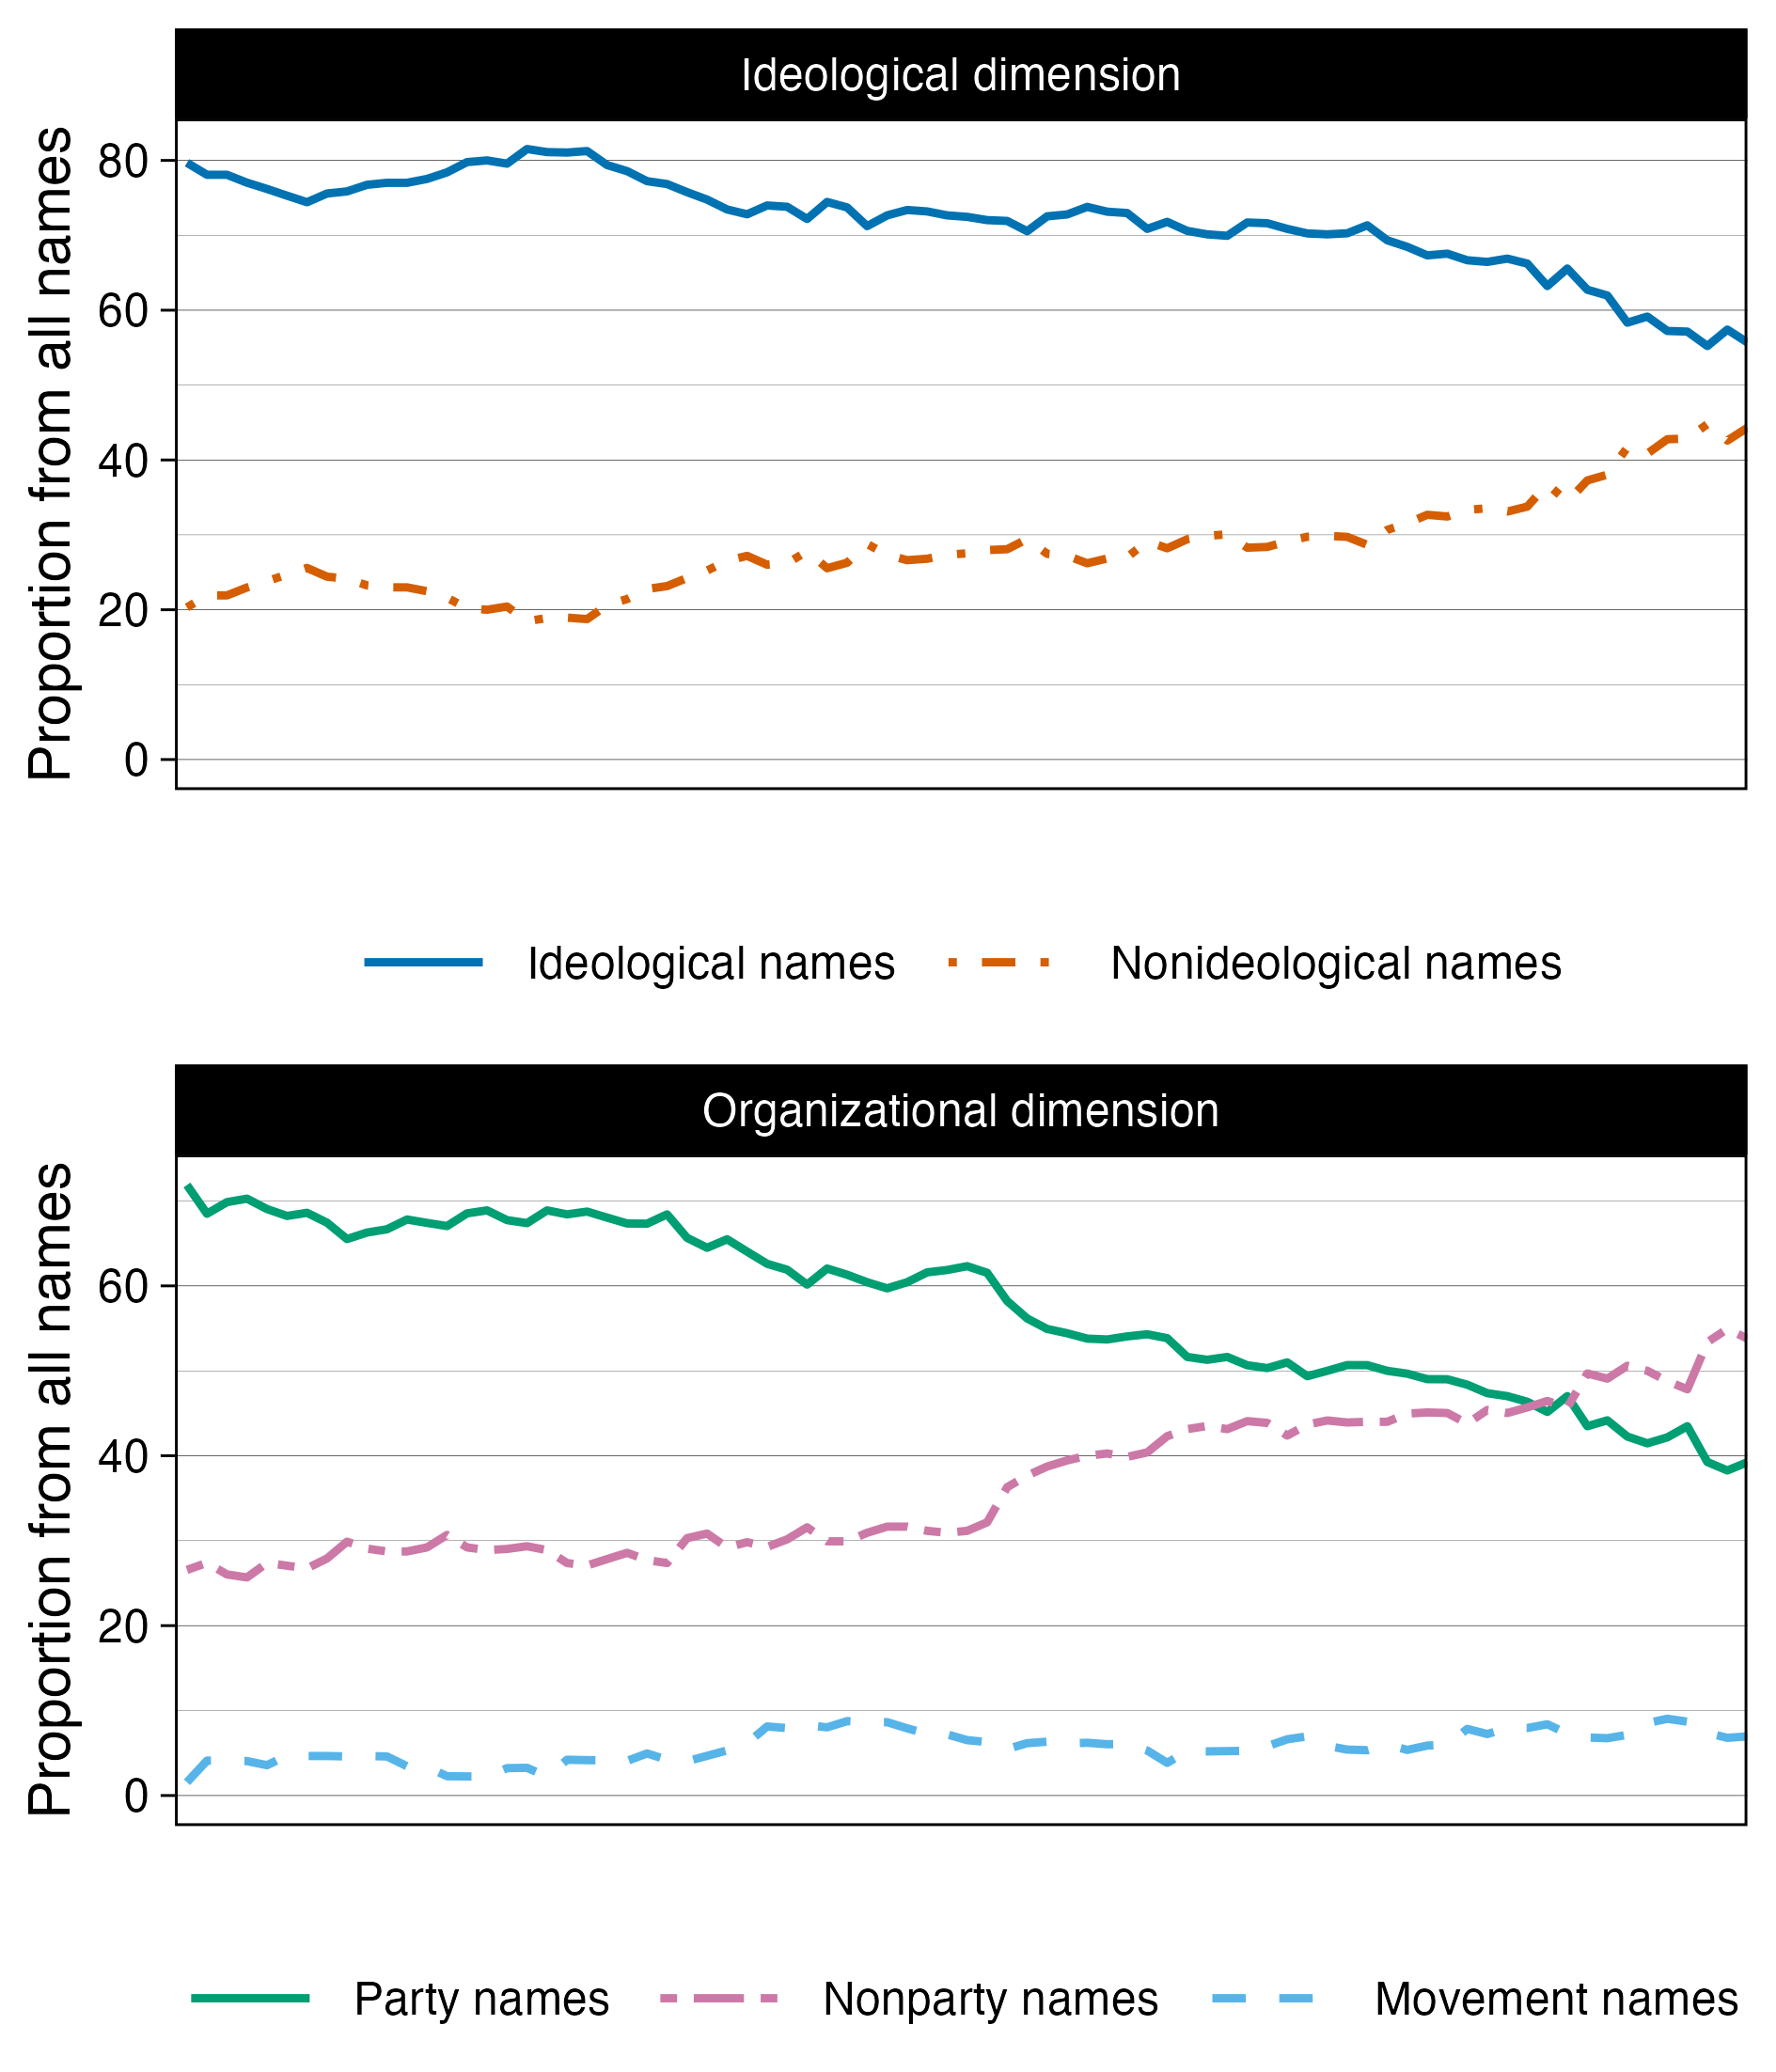
\includegraphics[width=0.9\textwidth]{./figures/Figure1.png} \caption{Distribution of party names over time (1945-2023)} \label{Fig:timeline} \floatfoot{Note: The figure shows the average trend across Western European countries. Appendix A Table 1 and Figure 4 shows the distribution by country.} \end{figure}

Contrary to the universal trends hypothesized by H1, movement references remain more marginal and develop in distinct waves. The data shows three peaks: 1950, 1978, and 2013. Each surge follows substantial turbulence in European protest and electoral politics. The first peak is explained by right-wing and Christian democratic parties taking up movement references in the immediate aftermath of the Second World War to rebrand the organization with a broader appeal. Prominent examples include the parties supporting General de Gaulle in France (People's Republican Movement, Rally for the Republic Group, Rally of Republican Lefts), the post-fascist Italian Social Movement, or the party of the fled/ expelled German minorities, the All-German Bloc. The second peak relates to the emergence of new social movements at that time and the related breakthrough of green parties, interacting strongly with street protests \citep[][]{Rohrschneider_1993}. The third peak captures the dynamic in southern Europe in the Great Recession, with new and existing  parties investing considerably into channeling protest mobilization for electoral purposes \citep[][]{della_Porta_et_al_2017}. During the same time, particularly post the so-called migration crisis in 2015/16, the radical right also branded itself by adopting social movement elements and investing in protest mobilization \citep[][]{Castelli_Gattinara_Pirro_2024}. Thus, adopting movement labels appears to be a strategic rebranding decision triggered by major upheavals rather than an ongoing or universal trends.\footnote{As Table 1 and Figure 4 in Appendix A demonstrate, take-up of nonideological movement references was primarily driven by national exposure to these patterns rather than by the less-country-specific trends associated with classical party names and nonideological nonparty references.} 

Next, we present the overall distribution of the six types of party names from our typology across all European countries (see Figure \ref{Fig:decision_tree}).

\begin{figure}[H] 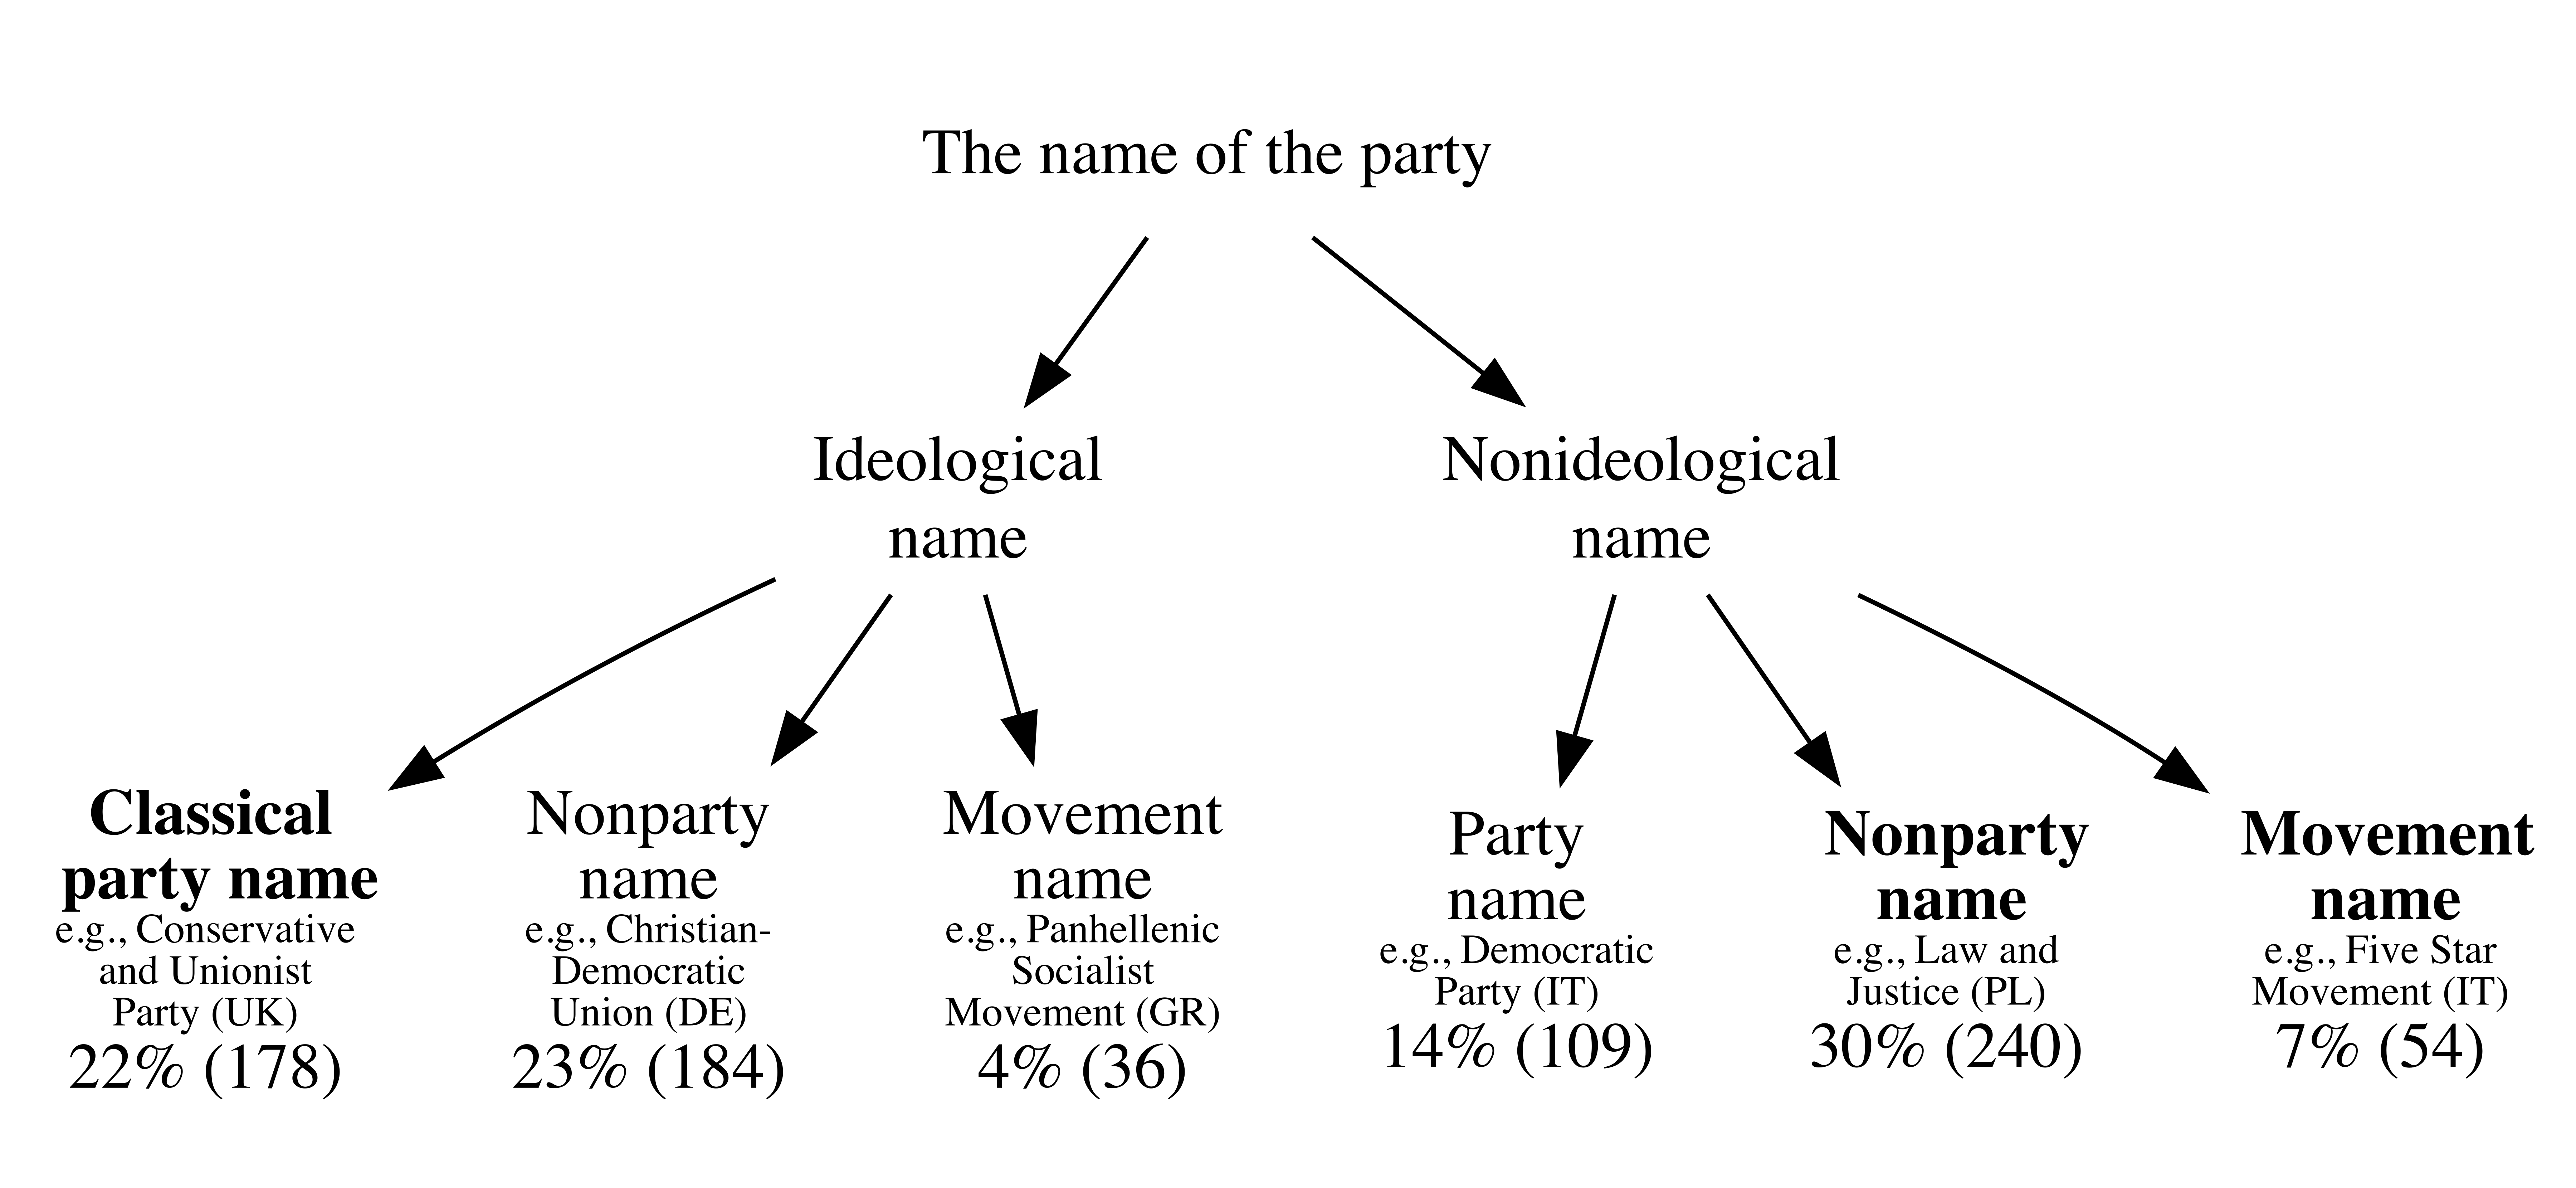
\includegraphics[width=\textwidth]{./figures/Figure2.png} \caption{Distribution of party name types in Europe} \label{Fig:decision_tree} \floatfoot{Note: All categories are mutually exclusive. The three types that we focus on are shown in bold.} \end{figure}

Only about a fifth of all party names in the dataset are classical (i.e., with both a traditional ideological and a party reference in their name). This underscores how dropping explicit ideology or the “party” label has become a strategic choice for many actors seeking broader or more innovative identities. Nonideological nonparty names, as a type of nonclassical name, constitute the largest single category, accounting for 30\% of all names. Examples include names with a reference to the country name (e.g., Forza Italia), values (e.g., Chasse, pêche, nature, traditions, meaning Hunting, Fishing, Nature, Traditions), a broad direction (e.g., the Danish Fælles Kurs, meaning Common Course), the name of the leader (e.g., Team Stronach), an action (e.g., Denk, meaning Think), or anti-elitism (e.g., La France Insoumise, meaning Insubordinate France). Movement names represent a significantly smaller share of party names. Ideological movement names are the rarest, with about 4\% of all names (e.g., Panhellenic Socialist Movement in Greece). Nonideological movement names are somewhat more frequent, with 7\% of all names. Examples include the Five Star Movement in Italy or the Mouvement Réformateur in Belgium.

Examining name changes for individual parties, we find that party names are remarkably stable; only around 17\% of parties in our dataset changed their name along either the ideological or organizational dimension. Name change appears more common when considering the more detailed, mutually exclusive six-category typology we develop: about 25\% of parties shifted between these categories. This is because the typology also captures cases that reflect unique combinations of changes across both dimensions. There are two particularly pronounced waves of party name changes: in the 1980s and the 2000s. We include additional analysis of these cases in Appendix B, which shows that the parties that change their name are fairly evenly distributed across the various parties and context-specific features we distinguish. Yet, the overall fairly low shares already hint at a central point of our argument: the observed shift in naming conventions at the party system level is not primarily driven by existing parties abandoning classical labels, but rather by the cumulative entry of new parties that choose nonclassical names from the outset.

\subsection{Party-level analysis}

To examine our expectations about party-level dynamics in more detail (H2), we begin by presenting the distribution of the three dependent variables by party family. Figure \ref{Fig:parfam_bar} shows the results. As the figure indicates, the choice between classical and nonclassical names largely follows a left-right divide: communist/socialist, social democratic, and green parties lean more toward classical, whereas liberal, conservative, and agrarian parties commonly pick nonideological or nonparty labels. Radical right parties often even adopt nonideological movement names.

\begin{figure}[H] 
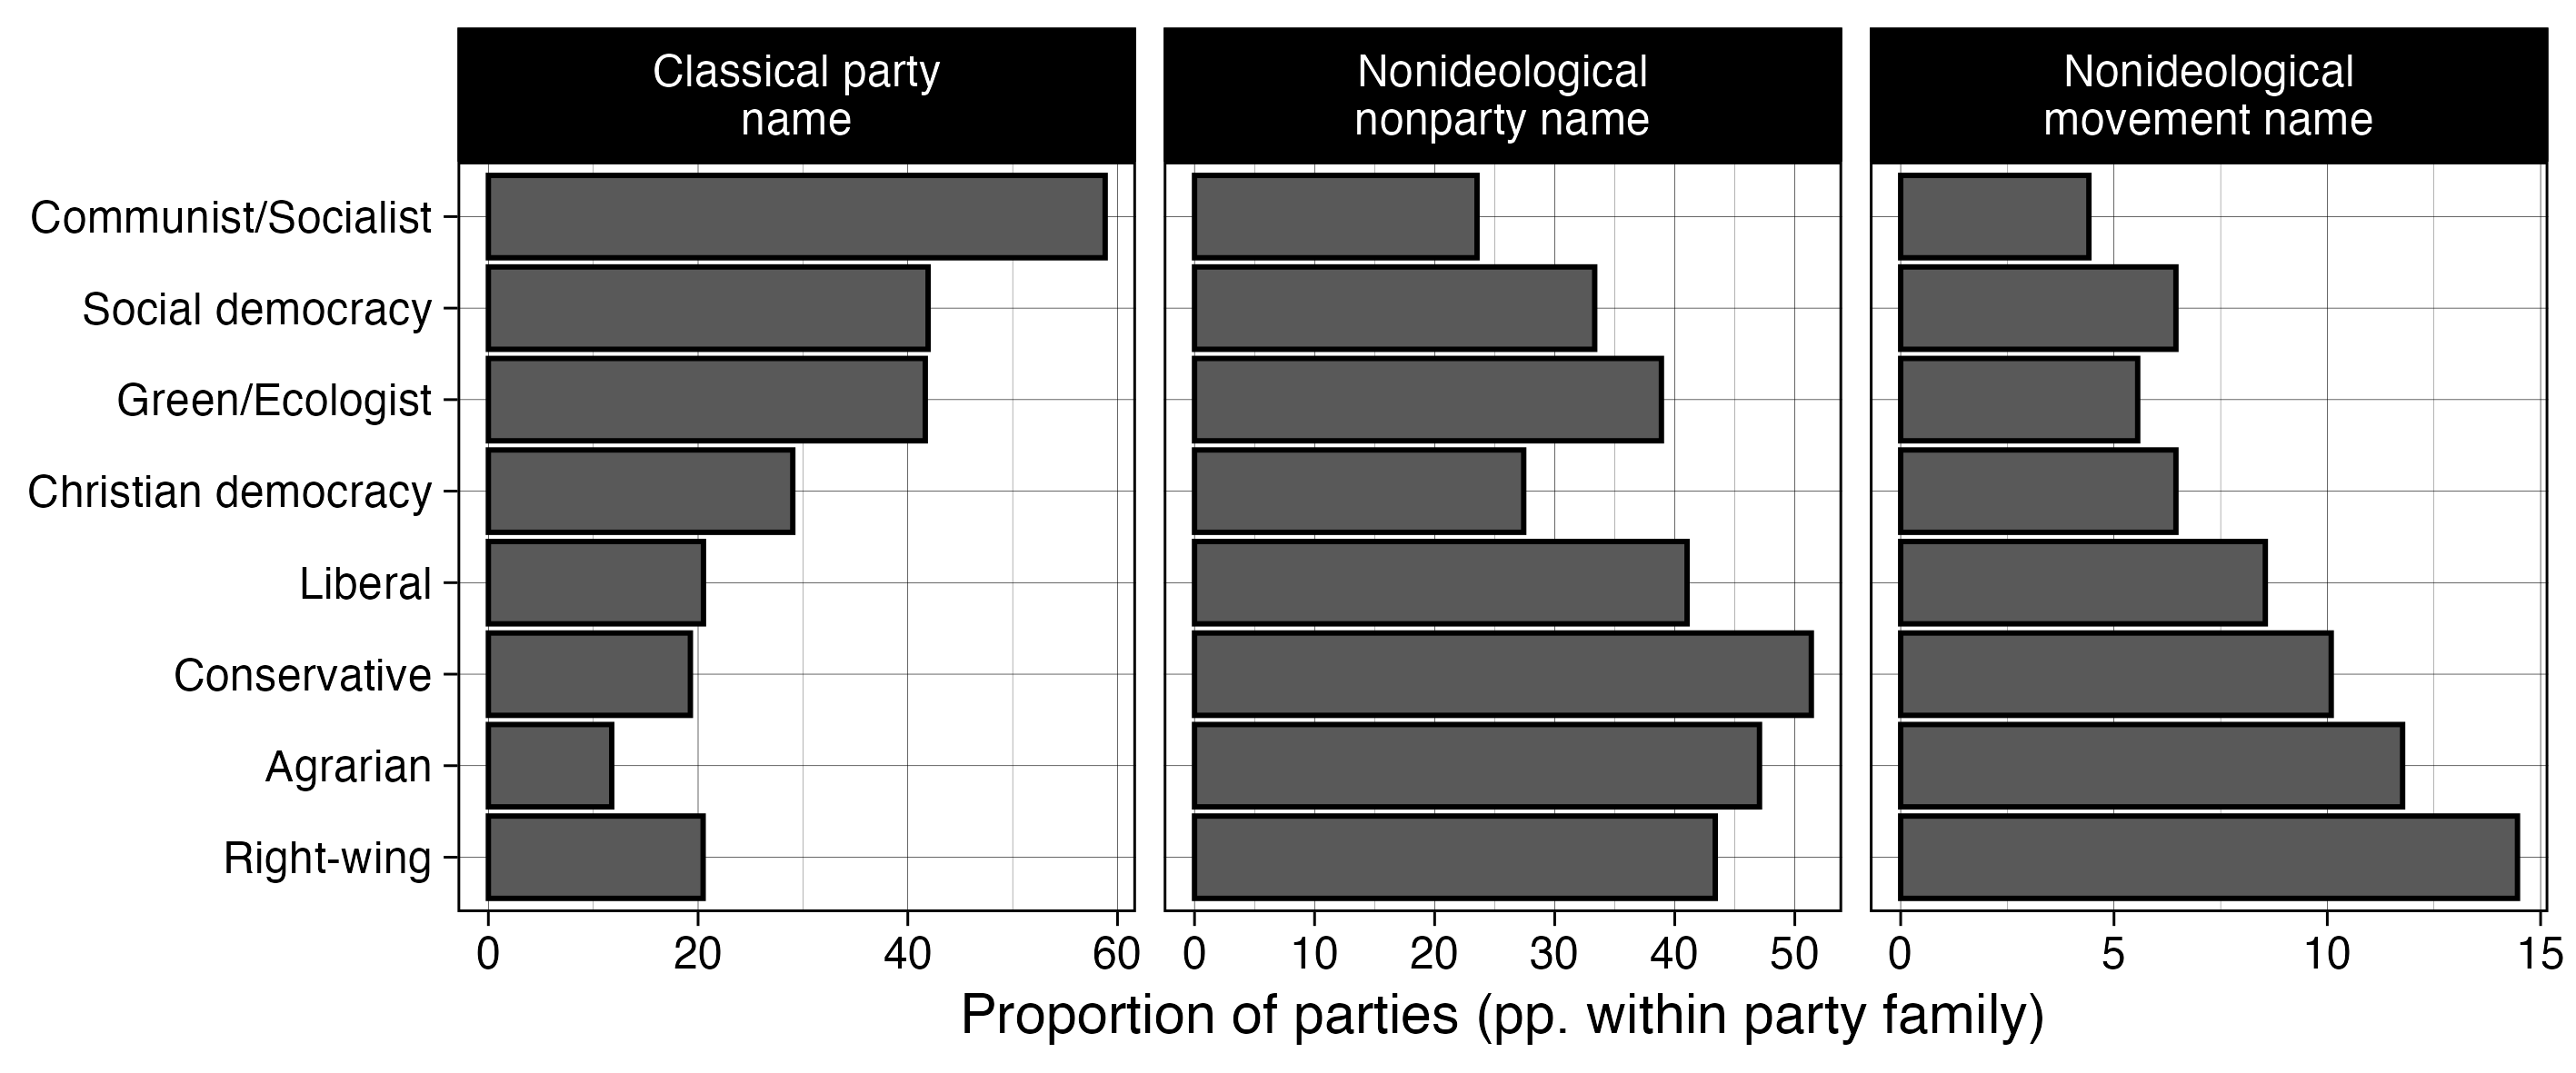
\includegraphics[width=\textwidth]{./figures/Figure3.png} 
\caption{Distribution of party names by party family (1945-2023)} 
\label{Fig:parfam_bar} 
\floatfoot{Note: The categories are mutually exclusive. See Figure \ref{Fig:decision_tree} for an overview of the typology.} 
\end{figure}

Next, Table \ref{tab:ttest_table} presents the distribution of names by party type using dichotomous indicators. Specifically, it shows how the three dependent variables vary among mainstream parties (mainstream party family: yes/no), parties that have previously held the prime ministership (yes/no), and new parties (yes/no). We consider a party ``new'' from the point at which it first secures at least 1 percent of the vote until the second election it contests.

\begin{table}[H]
\centering
\caption{\label{tab:unnamed-chunk-9}Distribution of brands by party type \label{tab:ttest_table}}
\centering
\begin{tabular}[t]{lr>{}rr>{}rr>{}r}
\toprule
\multicolumn{1}{c}{ } & \multicolumn{2}{c}{\makecell[c]{Classical \\ party \\ name}} & \multicolumn{2}{c}{\makecell[c]{Nonideological \\ nonparty \\ name}} & \multicolumn{2}{c}{\makecell[c]{Nonideological \\ movement \\ name}} \\
\cmidrule(l{3pt}r{3pt}){2-3} \cmidrule(l{3pt}r{3pt}){4-5} \cmidrule(l{3pt}r{3pt}){6-7}
\multicolumn{1}{c}{ } & \multicolumn{1}{c}{Share} & \multicolumn{1}{c}{Diff.} & \multicolumn{1}{c}{Share} & \multicolumn{1}{c}{Diff.} & \multicolumn{1}{c}{Share} & \multicolumn{1}{c}{Diff.} \\
\cmidrule(l{3pt}r{3pt}){2-2} \cmidrule(l{3pt}r{3pt}){3-3} \cmidrule(l{3pt}r{3pt}){4-4} \cmidrule(l{3pt}r{3pt}){5-5} \cmidrule(l{3pt}r{3pt}){6-6} \cmidrule(l{3pt}r{3pt}){7-7}
Mainstream party family & 26.7 & -2.9 & 31.0 & -0.8 & 9.8 & -0.9\\
Challenger party family & 29.7 &  & 31.7 &  & 10.7 & \\
Previously PM party & 35.8 & 7.8 & 23.1 & -8.4 & 9.9 & 0.1\\
Previously no PM party & 28.0 &  & 31.5 &  & 9.8 & \\
New party & 26.6 & -4.2 & 29.2 & 1.9 & 9.4 & -0.2\\
Existing party & 30.8 &  & 27.3 &  & 9.6 & \\
\bottomrule
\multicolumn{7}{l}{\rule{0pt}{1em}Note: The values are averaged across all countries.}\\
\end{tabular}
\end{table}


Overall, these party-specific characteristics exhibit the expected associations, but party family stands out as an exception. As shown above, mainstream vs. challenger party families do not fully account for differences in classical versus nonclassical names. Indeed, parties in challenger families score higher not only on classical party names but also on nonideological nonparty and nonideological movement names.\footnote{This result is partly driven by the Eastern European pattern, where mainstream parties are generally more likely to adopt nonclassical names (see Figures 3 and 5, as well as Tables 1 and 4 in Appendix C).} Not having held the prime ministership substantially affects two of the three dependent variables in the anticipated direction: parties that have served as prime ministers are more likely to adopt a classical party name and less likely to choose a nonideological nonparty name. Similarly, new parties are less likely to select a classical party name and more likely to opt for a nonideological nonparty name. 

\subsection{Multilevel regression model}

Because some of these factors are correlated (see Appendix A, Figure 5), we now turn to the multivariate regression analysis to estimate their marginal effects and formally test our hypotheses. The regression model includes controls for logged party age, vote share, electoral coalitions, and opposition status, plus all previously introduced contextual variables. \footnote{Except for logged party age and electoral coalitions, all independent variables are lagged by one election. All independent variables are rescaled to range between 0 and 1 so that their effect sizes are directly comparable. Party-level variables are group-centered around the country*year mean, and country*year-level contextual features are centered around each country's mean \citep{Enders_Tofighi_2007}.} Figure \ref{Fig:mlm_results} presents the results with estimated average marginal effects.

\begin{figure}[H] 
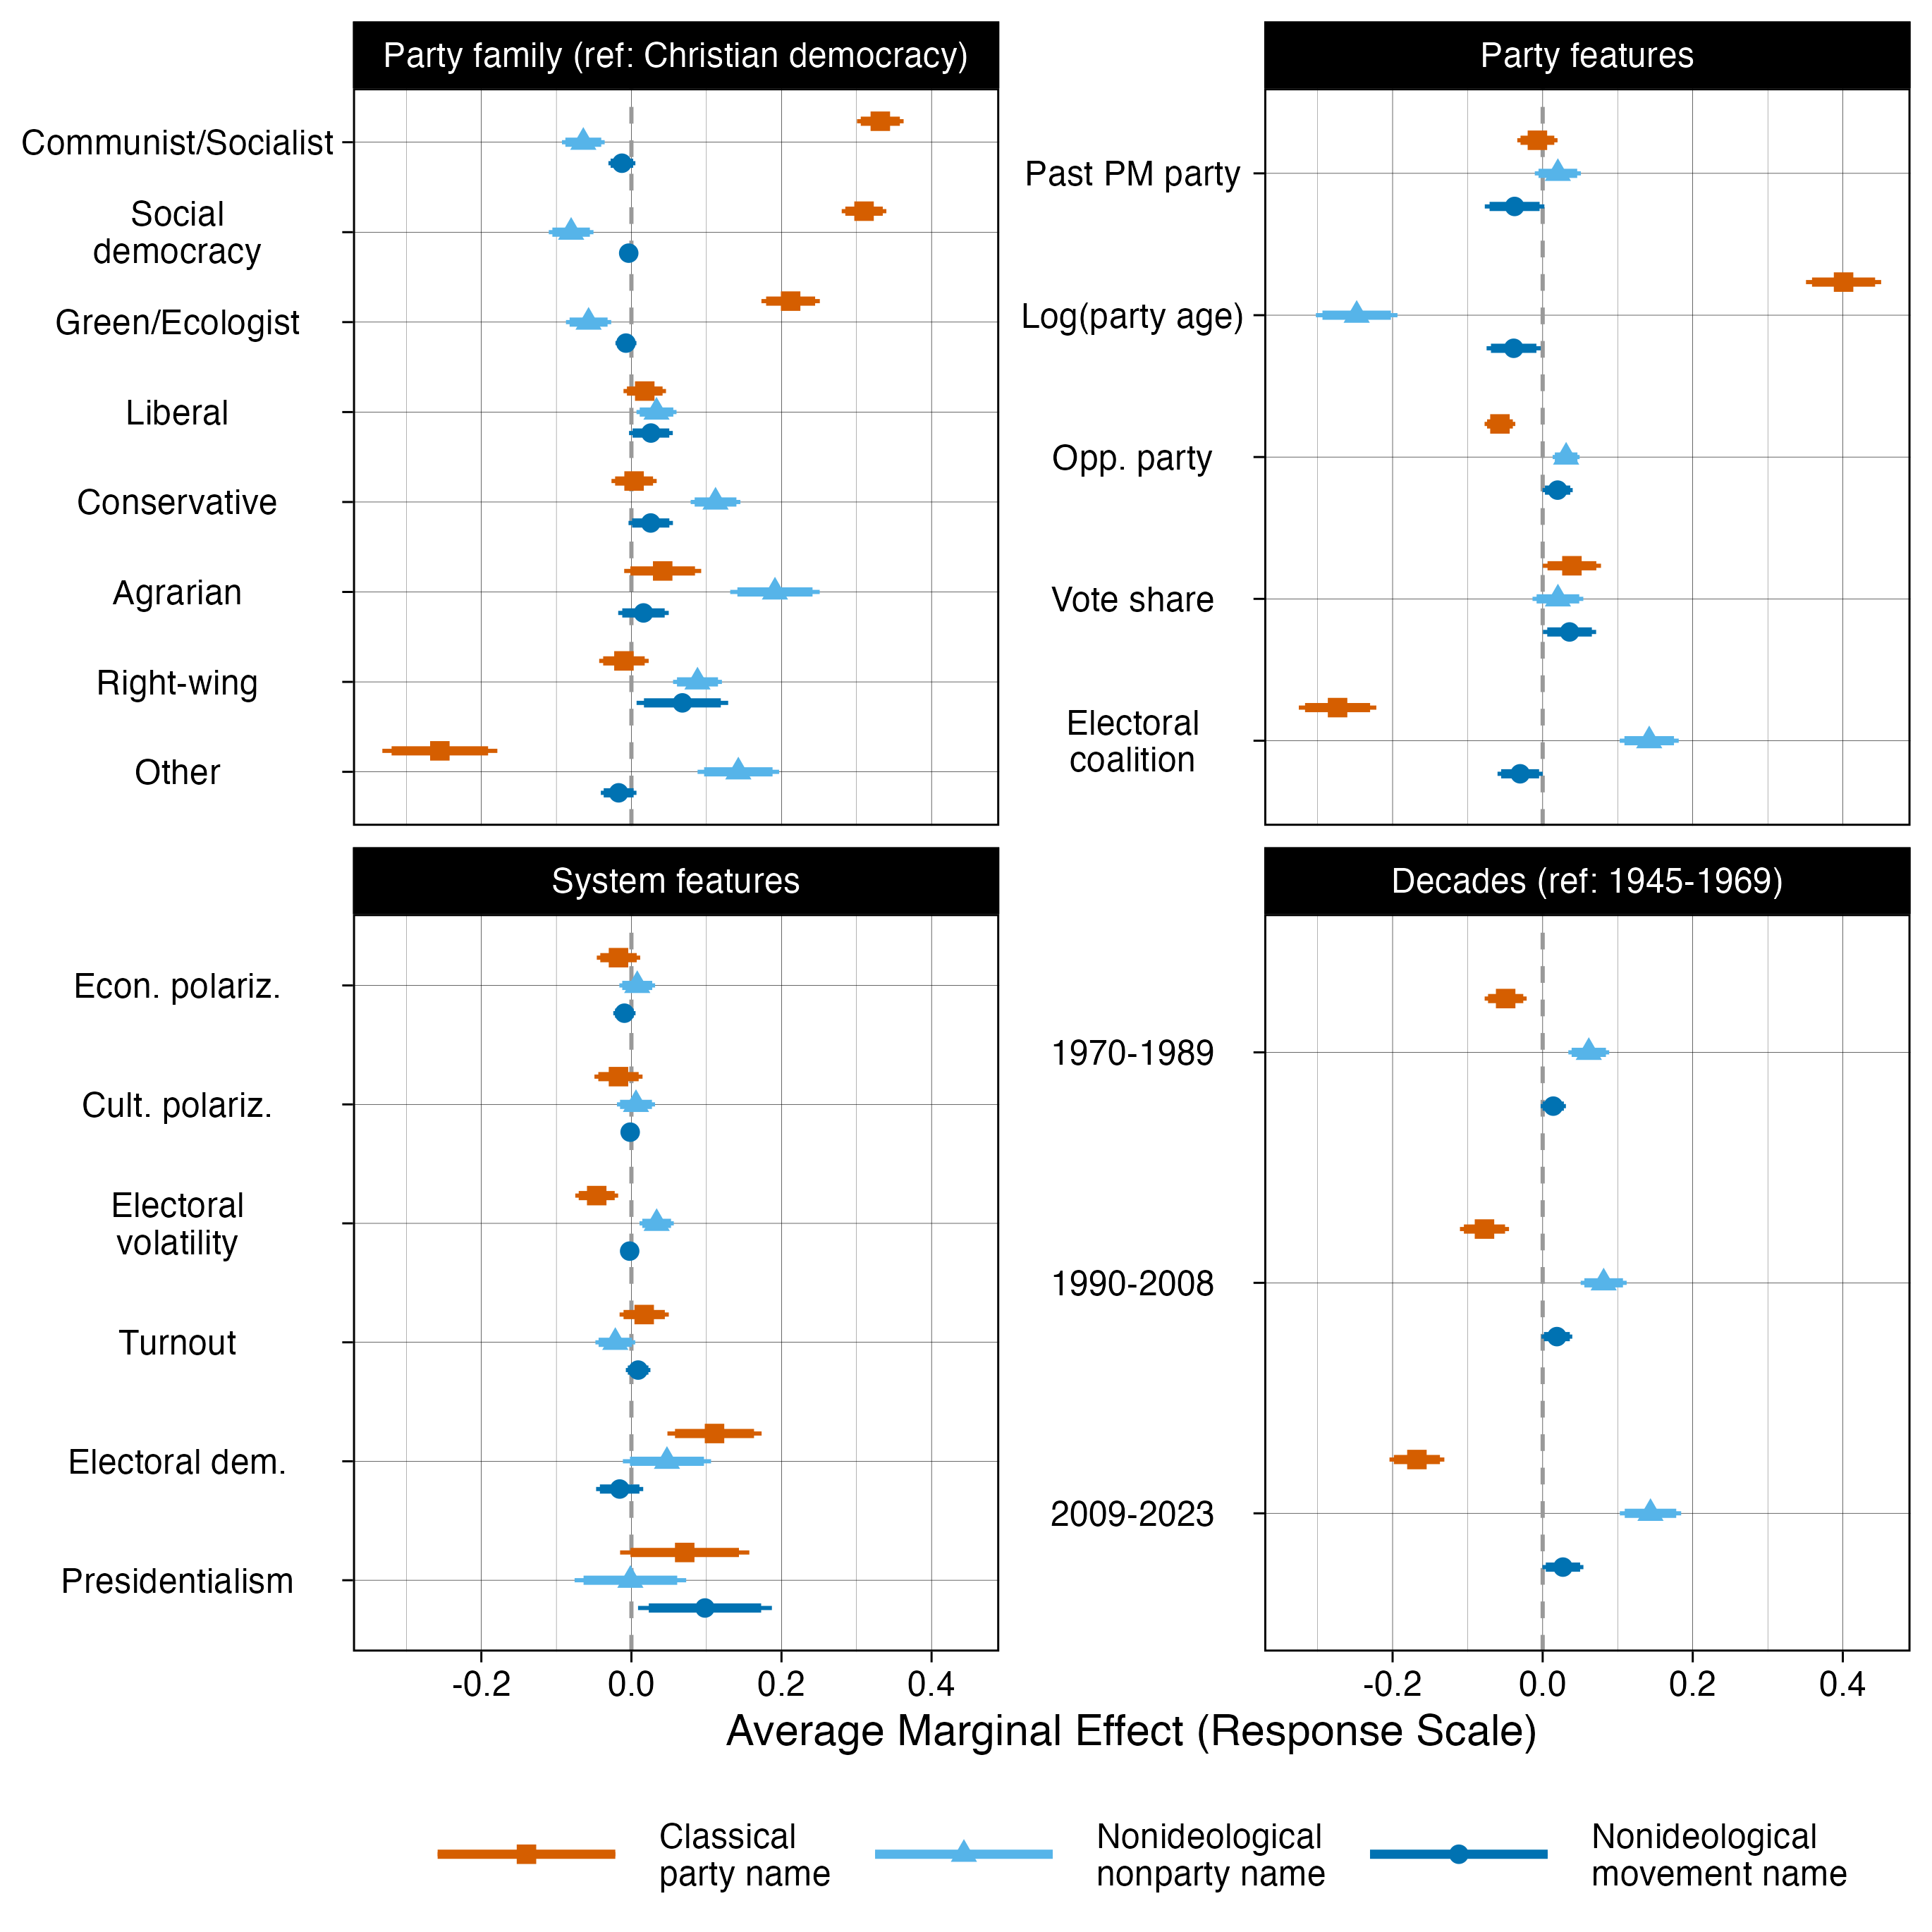
\includegraphics[width=\textwidth]{./figures/Figure4.png} 
\caption{Logistic regression model of party naming} 
\floatfoot{\textit{Note:} Estimates are from the full sample shown in Appendix A, Table 2. Thick error bars represent 90\% confidence intervals; thin error bars represent 95\% confidence intervals. The model is a three-level logistic regression with random intercepts, nesting observations within country*years and countries.} 
\label{Fig:mlm_results} 
\end{figure}

These findings provide further nuance to what we observed in the bivariate analysis. Regarding party-family effects, the results offer additional support for the left-right differences noted earlier. Contrary to the bivariate analysis, once we control for party family, opposition status, and vote share, parties that held the prime ministership mainly differ by being less likely to use a nonideological movement name. Overall, party age is the strongest predictor: older parties are much more likely to retain classical party names and much less likely to pick nonclassical ones. This aligns with our descriptive findings, indicating that only a tiny minority of established parties rebrand themselves. Therefore, nonclassical names predominantly emerge when new parties enter the system.

Regarding the control variables, opposition parties are less likely to have a classical party name and more likely to adopt nonideological nonparty or nonideological movement names. Vote share positively predicts all three name types (with the smallest effect on nonideological movement names). Electoral coalitions are less likely to use a classical or nonideological movement name but more likely to use nonideological nonparty name.

Overall, left-right ideology, newness, and, partially, opposition status drive the likelihood of adopting nonclassical names. In contrast, the mainstream-challenger divide in terms of programmatic offer does not match the expectations, as green parties cluster with other parties from the left. Thus, we cannot fully confirm H2.

Among the contextual variables, polarization, linked to the structuralist perspective, has no effect on party names. By contrast, electoral volatility, linked to the functionalist perspective, shows a statistically significant negative association with classical party names and a positive one with nonideological nonparty names. Yet, volatility is not related to the uptake of nonideological movement names. Turnout has also no statistically significant relationship with any of the three name types. Meanwhile, higher levels of electoral democracy are positively associated with classical party names, and presidentialism predicts using nonideological movement names.

Considering all these party-level and contextual variables, classical party names decrease in prevalence over time, while nonclassical names become more common. This trend is strongest for nonideological nonparty names and relatively weaker for nonideological movement names. Overall, these patterns align with the descriptive results, supporting H1.

\subsection{Survey experiments}

Finally, we turn to the survey experiment to explore how party names affect electoral appeal. As noted, our survey experiment varied the name of a new party entering parliament that aligned programmatically with respondents' preferences. We also examined the effect of party organization and mobilization repertoire, which serve as reference points. We present only the main effects here and include further analyses in Appendix E. Figure \ref{conjoint1_main} shows the average marginal component effects of different party names on a new party's electoral appeal.

\begin{figure}[H] 
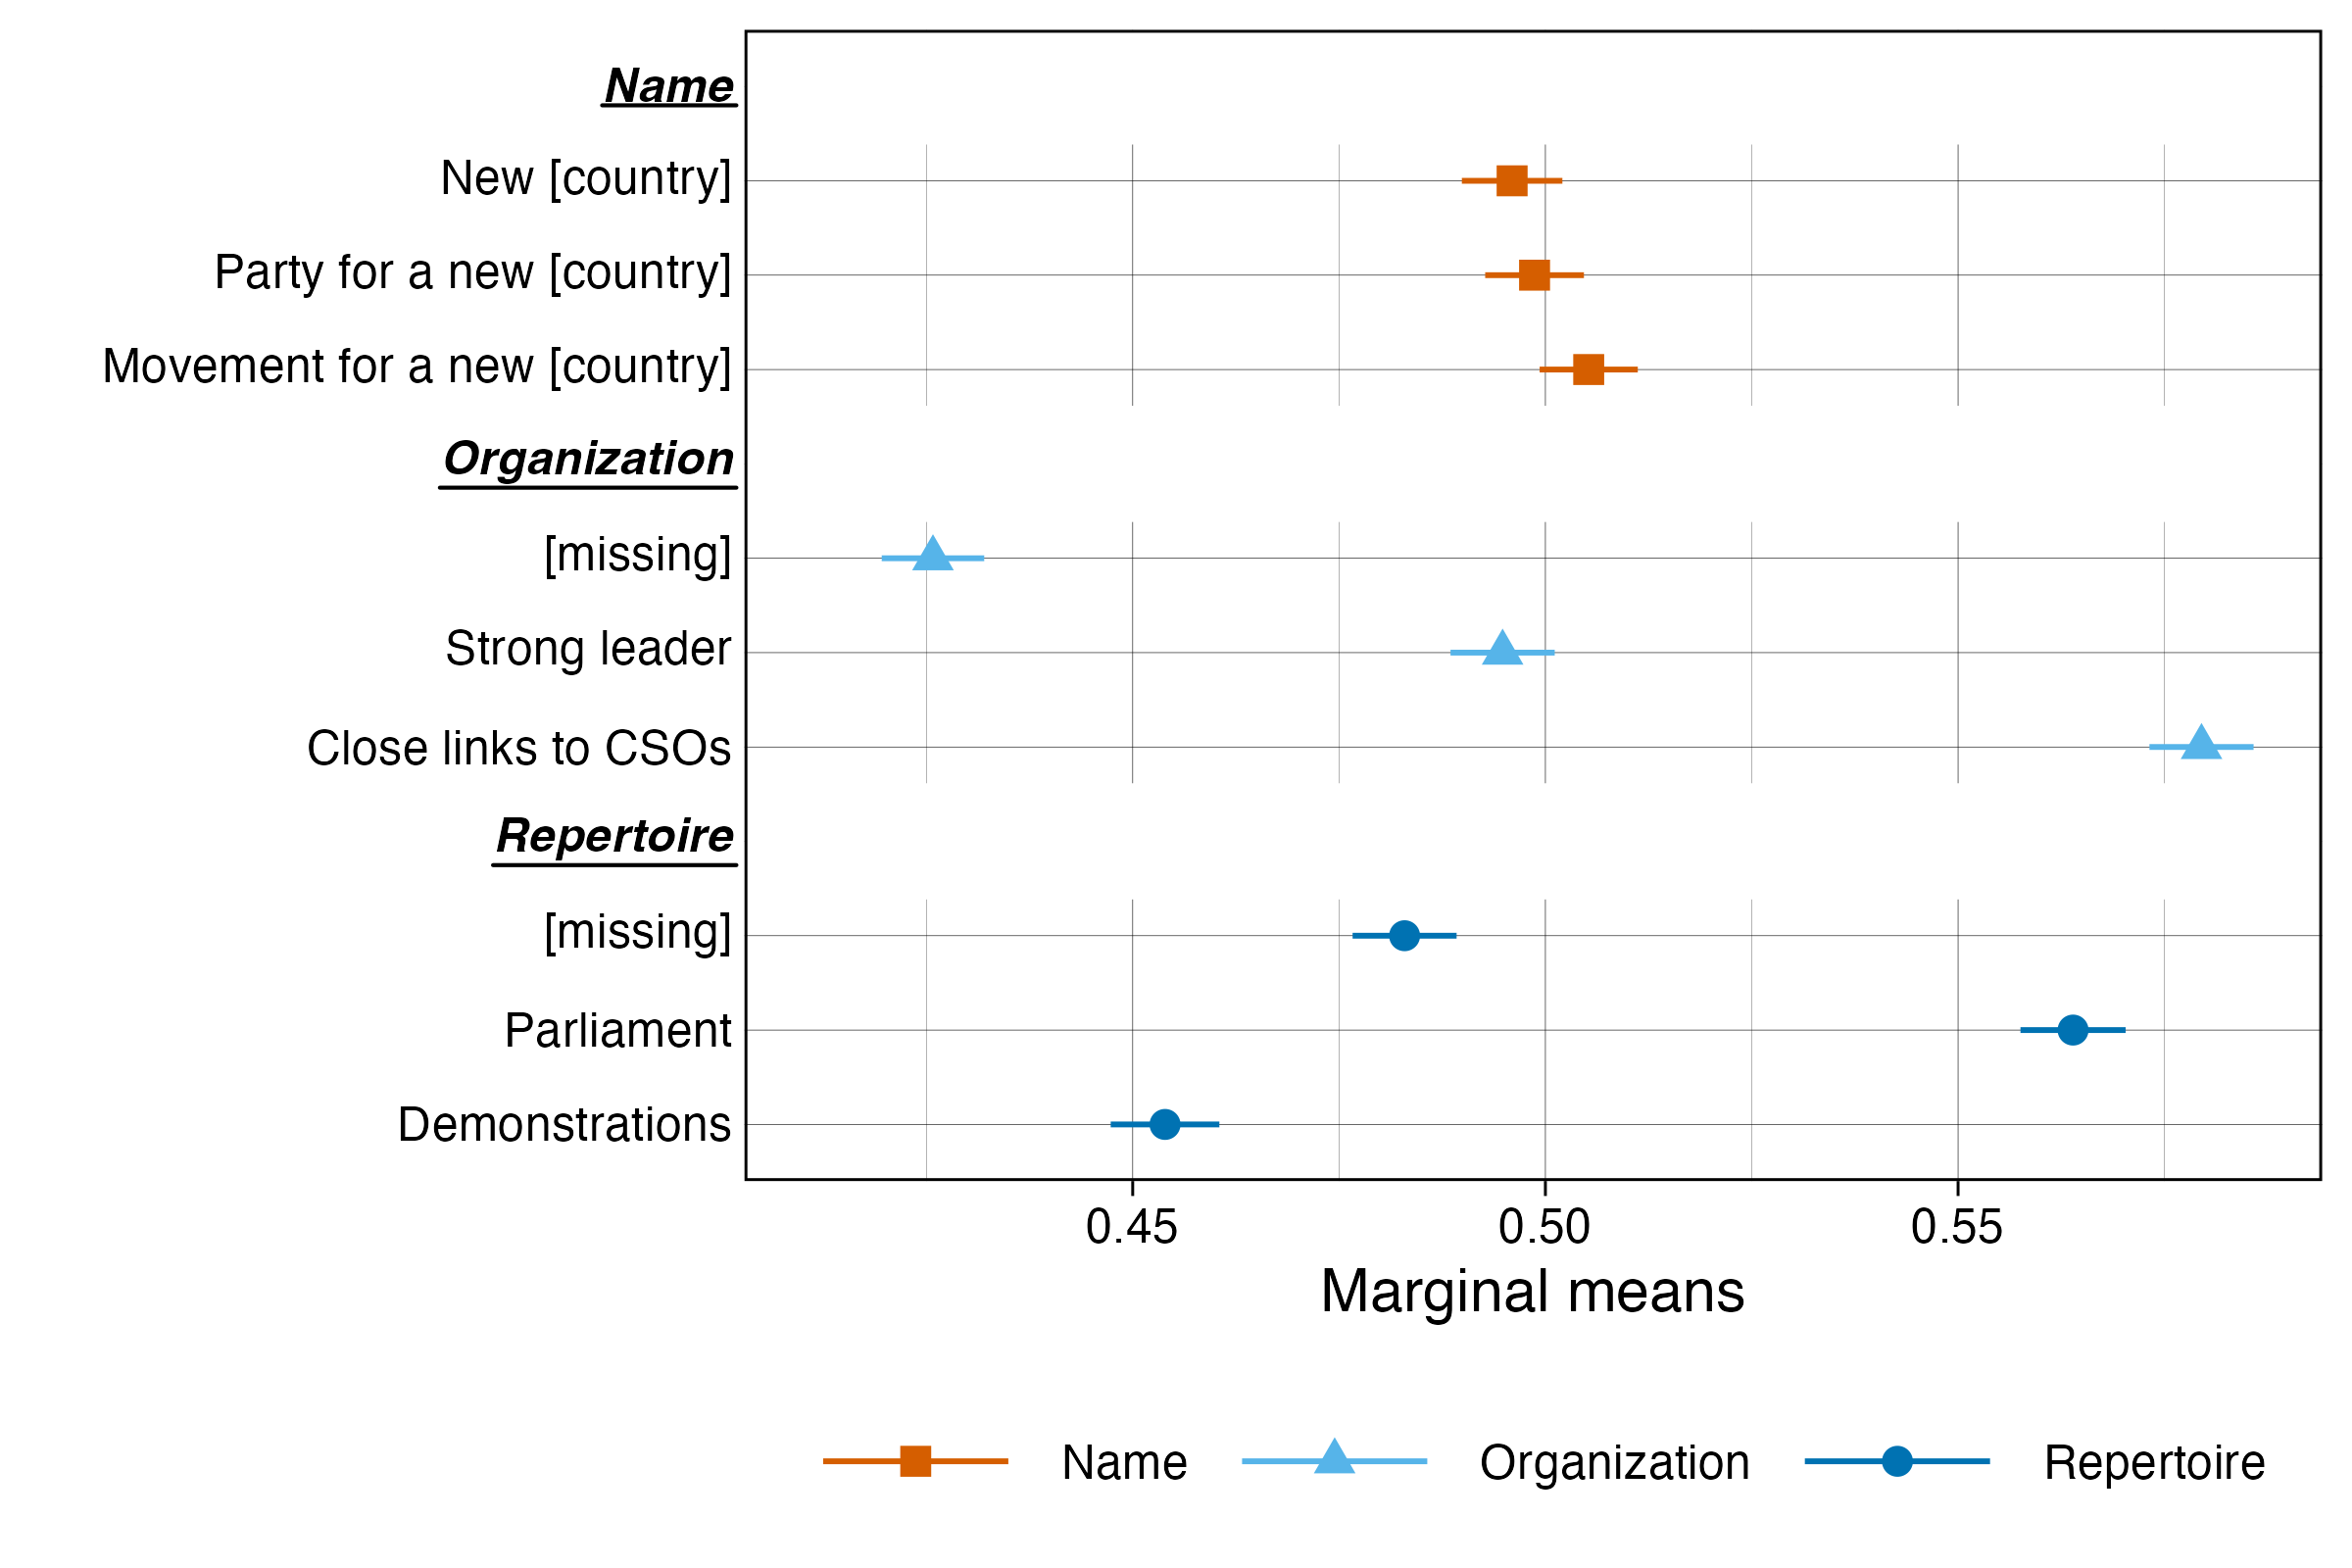
\includegraphics[width=\textwidth]{./figures/Figure5.png} 
\caption{New party branding conjoint experiment} 
\floatfoot{\textit{Note:} The error bars represent 95\% confidence intervals. The model is specified with standard errors clustered by respondent ID.} 
\label{conjoint1_main} 
\end{figure}

Contrary to our expectation (H3), the effect of party names on a new party’s electoral appeal is negligible. Compared to having no organizational label, explicitly calling the group a ``party'' does not reduce its popularity. A movement name does lead to a statistically significant increase in appeal relative to no organizational label. Yet, the difference is only about one percentage point from no organizational reference or the word ``party''. Some cross-country differences arise (e.g., Hungary and Germany, as shown in Appendix D and E), but overall, nonclassical naming does not produce a notable boost.

Instead, the results from the conjoint experiment indicate that voters reward strong leadership and close ties with civil society.  Voters also prefer parties that focus on parliamentary work rather than organizing public demonstrations, suggesting that ``taking the fight to the streets'' is generally not that appealing to voters.

Thus, we do not find sufficient evidence to confirm H3, which posits that nonclassical names boost electoral appeal compared to classical names.\footnote{In our second experiment, we test the effect of a name change based on the respondent's own party. The experiment presents a counterfactual scenario in which the respondent's party either drops or adds a ``party'' or ``movement'' to its name. Results show that name changes consistently decrease electoral support. Party organization and mobilization repertoire attributes have similar effects. See Appendix D, Figure 2, and Appendix E for details.} We also find no strong evidence for heterogeneity across various respondent-level attributes, only issue salience regarding climate as compared to taxation, welfare, or immigration somewhat increases the appeal of ``movement'' or ``party'' labels over no label. (see Figure 27, Appendix E).\footnote{For the party rebranding experiment, we find more heterogeneous effects, largely aligned with our preregistered expectations.}

In sum, our findings suggest that despite the growing prevalence of nonclassical names, voter preferences are more influenced by party leadership and  to civil society than by naming practices. Nonclassical names do differentiate parties symbolically, but other factors appear more decisive in shaping support among the electorate.

\section{Conclusion} 

The current paper is the first study to systematically describe and explain the transformation of party brands in Europe, as captured by the dynamic of changing party names. We make at least three contributions by (i) introducing a content-based perspective, (ii) examining developments in the electoral arena in interaction with the rise of movement-based mobilization, an (iii) identifying the causal effects of party names on a party's electoral appeal.

The empirical results point to an apparent paradox. Despite a pronounced shift away from classical party names toward nonclassical names that lack both an ideological and a party reference, nonclassical names are not particularly rewarded by the electorate. We shows that, on the supply side of party names, especially since the late 1960s, nonideological nonparty names have become the most prevalent form of self-identification for political parties. Parties that embrace nonclassical names tend to be newly founded ones, especially on the right and in opposition. Some parties, particularly during broad protest waves, went further and adopted nonideological movement names. This uptake of nonideological movement names is particularly prevalent among the radical right. Our hierarchical regression models indicates that volatility, the main indicator associated with the functionalist perspective on the crisis of parties, predicts the uptake of nonideological nonparty and movement names.

Turning to the demand side, the conjoint experiments demonstrate that party names do not have a substantively significant effect on a new party's appeal, and that renaming, regardless of content, is generally punished. Despite this paradoxical result, the survey experiments also show that the electorate rewards some aspects of nonclassical brands. In particular, if parties adopt organizational structures that foster closer links to civil society, they can increase their electoral appeal. Other aspects of movement brands, such as organizing demonstrations instead of focusing on parliamentary work, are not rewarded by the electorate.

We want to highlight two implications of our empirical findings. First, the fact that right-wing parties drive the upatake of nonclassical brands underscores the continuing importance of ideological differences alongside the emerging mainstream-vs.-challenger party divide. This partly challenges the canonical literature on the decline of ideology in the postwar era (dominated by catch-all parties) and points to a new facet of party competition that is often overlooked. Namely, left- and right-wing parties do not only compete on programmatic grounds; they also compete through their brands. More specifically, the two types of formations differ (a) in the extent to which their brands remain integrated into postwar ideological antagonisms and (b) in the extent to which they offer organizational forms outside classical models of party governance. With respect to these two dimensions of their brand, left-wing parties tend to be more conservative, which is, at least partly, in line with the preferences of the electorate.

Second, the results warn against applying off-the-shelf solutions that assume nonclassical branding automatically confers a competitive advantage. European electorates have a nuanced perspective on the crisis of representation: they do not take cues solely from party names but also from organizational form and action repertoire. While citizens expect parties to cooperate with civil society organizations, they still want them to focus on parliamentary representation instead of organizing demonstrations. They also prefer that established parties retain their existing brands, as shown by the negative effects of renaming. Future research on the citizen side should go beyond the hypothetical setup of our experiment by studying specific (re)branding decisions using panel data and by theorizing and testing the conditions under which classical and nonclassical names might be electorally beneficial rather than considering only direct effects.

Based on our results, we also propose an optimistic interpretation: although the decline of classical party names on the supply side and voters' relative indifference to newly emerging labels could signal a crisis of parties, it has not (yet) led to a deep-seated disenchantment with classical brands. Instead, our results suggest that voters continue to demand that parties deliver effective representation in national parliaments. Future research should also explore whether the uptake of nonclassical names diffuses through party families or across levels of governance, including the European level. Investigating diffusion dynamics and family effects could clarify how naming conventions are shaped by transnational political alignments and institutional contexts.

\singlespacing

\bibliography{bibliography.bib}

\end{document}